\begin{example}
	Suppose a chemical reaction produces higher yields of a product, the higher the ambient temperature
	\begin{center}
		\begin{tikzpicture}
		\begin{axis}[
		xmin=50, xmax=100, xlabel=temperature,
		ymin=100, ymax=250, ylabel=yiels,
		samples=400,
		axis x line=bottom,
		axis y line=left,
		domain=50:100,
		]
		\addplot[mark=x,only marks] coordinates {
			(50,120)
			(53,115)
			(54,125)
			(55,119)
			(56,120)
			(59,140)
			(62,145)
			(64,143)
			(67,147)
			(71,157)
			(72,160)
			(74,175)
			(75,159)
			(76,177)
			(79,180)
			(80,185)
			(82,182)
			(85,185)
			(87,188)
			(89,200)
			(93,195)
			(94,203)
			(95,204)
			(97,212)
		};
		\end{axis}
		\end{tikzpicture}
	\end{center}
	Simple linear regression is what we can use to investigate if a relationship between two variables exists when we don't know about the underlying process. We model a linear relationship between two variables and
	\begin{enumerate}[label=(\alph*)]
		\item quantify this pattern before
		\item testing if we can believe it
	\end{enumerate}
\end{example}

\subsection{Structure of simple linear regression models}

\begin{definition}[simple linear regression]
	For $n$ observed data pairs $\{(x_i,Y_i)\mid i=1,...,n\}$ \begriff{simple linear regression} assumes we have the relationship
	\begin{align}
		Y_i = \beta_0 + \beta_1x_i + \epsilon_i\notag
	\end{align}
	$Y$ is called the \begriff{respose variable} and $x$ the \begriff{explainatory variable}. $\beta_0$ and $\beta_1$ are \begriff{model parameters}. $\epsilon_i$ are error terms (spread around the regression line) and crucially, we assume $\epsilon_i\overset{i.i.d}{\sim}Normal(0,\sigma)$ in simple linear regression.
\end{definition}

\begin{definition}[alternative representations for simple linear regression models]
	\begin{enumerate}[label=(\alph*)]
		\item algebraic notation:
		\begin{align}
			Y_1 &= \beta_0 + \beta_1x_1 + \epsilon_1 \notag \\
			Y_2 &= \beta_0 + \beta_1x_2 + \epsilon_2 \notag \\
			\vdots  \notag \\
			Y_n &= \beta_0 + \beta_1x_n + \epsilon_n \notag
		\end{align}
		\item Matrix notation:
		\begin{align}
			Y = \beta X + \epsilon \notag 
		\end{align}
		Because of the error term $\epsilon$, the response $Y$ is a random variable. So, $Y_i = E(Y_i)+\epsilon_i = \beta_0+\beta_1x_i+\epsilon_i$ and thus $E(Y_i) = \beta_0+\beta_1x_i$. This leads to the following notation
		\item Random variable notation: 
		\begin{align}
			Y_i &\overset{i.i.d}{\sim}Normal(\beta_0+\beta_1x_i,\sigma) \notag \\
			Y &\sim Normal(X\beta,\mathbbm{1}\sigma) \notag
		\end{align}
		Since the mean of the response is a linear function of the explanatory variables, there are often called \begriff{simple linear models}.
	\end{enumerate}
\end{definition}

Given data, we want to estimate the parameters of the model. In this course, we always use Maximum Likelihood Estimation (MLE). That means, we find parameter values that maximise the likelihood of our model. The likelihood for an simple linear model is
\begin{align}
	L(\beta\mid X) = \prod_{i=1}^{n} f_{Normal}(Y_i,\mu=\beta_0+\beta_1x_i,\sigma) \notag
\end{align}
where $f_{Normal}$ is the PDF for the normal distribution with mean $\mu=\beta_0+\beta_1x_i$ and standard deviation $\sigma$ evaluated at $Y_i$. For linear models, it has been shown that MLE is equivalent to Ordinary Least Squares (OLS). For linear models exact equations for these parameter estimates exist
\begin{align}
	\hat{\beta} &= (X^TX)^{-1}X^TY \notag \\
	\hat{\sigma}^2 &= \frac{1}{n-2}(Y-X\hat{\beta})^T(Y-X\hat{\beta})\notag
\end{align}
Fitted values for the response are: $\hat{Y} = X\hat{\beta}$

\begin{center}
	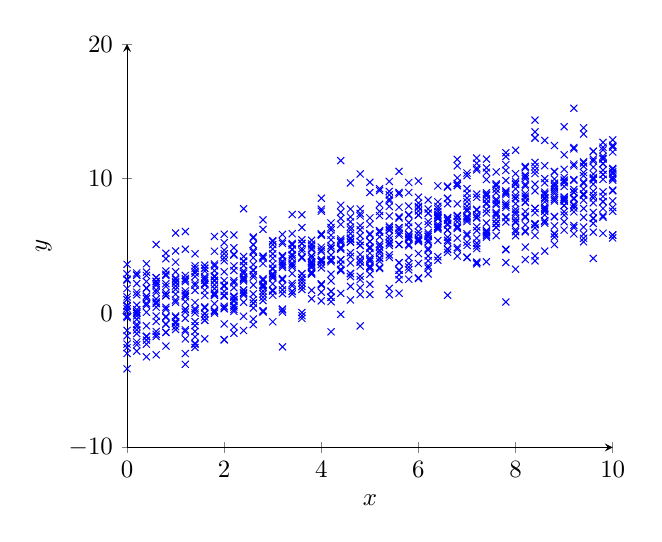
\begin{tikzpicture}[scale=0.9]
	\begin{axis}[
	xmin=0, xmax=10, xlabel=$x$,
	ymin=-10, ymax=20, ylabel=$y$,
	samples=400,
	axis x line=bottom,
	axis y line=left,
	domain=0:-10,
	]
	\addplot[mark=x,only marks, blue] coordinates {
		(0.00,-3.01)
		(0.00,3.62)
		(0.00,-0.23)
		(0.00,2.45)
		(0.00,0.99)
		(0.00,1.82)
		(0.00,-2.31)
		(0.00,2.52)
		(0.00,2.91)
		(0.00,-4.15)
		(0.00,-0.35)
		(0.00,-1.30)
		(0.00,0.31)
		(0.00,-1.70)
		(0.00,0.56)
		(0.00,1.19)
		(0.00,0.49)
		(0.00,-0.24)
		(0.00,-2.58)
		(0.00,0.12)
		(0.20,-0.84)
		(0.20,-2.36)
		(0.20,0.09)
		(0.20,-0.22)
		(0.20,0.58)
		(0.20,2.18)
		(0.20,1.35)
		(0.20,2.81)
		(0.20,-1.26)
		(0.20,-1.53)
		(0.20,0.01)
		(0.20,2.97)
		(0.20,2.81)
		(0.20,-0.05)
		(0.20,-0.99)
		(0.20,-2.84)
		(0.20,1.54)
		(0.20,0.25)
		(0.20,-2.16)
		(0.20,-0.47)
		(0.40,-3.26)
		(0.40,1.26)
		(0.40,0.05)
		(0.40,3.66)
		(0.40,-2.32)
		(0.40,2.34)
		(0.40,0.69)
		(0.40,0.57)
		(0.40,1.83)
		(0.40,2.79)
		(0.40,-1.74)
		(0.40,3.04)
		(0.40,-2.02)
		(0.40,-1.75)
		(0.40,-0.95)
		(0.40,1.87)
		(0.40,-1.74)
		(0.40,1.07)
		(0.40,1.22)
		(0.40,0.71)
		(0.60,1.71)
		(0.60,-1.75)
		(0.60,2.62)
		(0.60,0.83)
		(0.60,2.06)
		(0.60,-1.37)
		(0.60,0.70)
		(0.60,2.36)
		(0.60,2.63)
		(0.60,0.43)
		(0.60,-3.11)
		(0.60,-1.59)
		(0.60,1.04)
		(0.60,2.19)
		(0.60,1.53)
		(0.60,-0.63)
		(0.60,5.09)
		(0.60,0.74)
		(0.60,2.33)
		(0.60,-0.23)
		(0.80,-1.43)
		(0.80,2.17)
		(0.80,2.88)
		(0.80,4.44)
		(0.80,-0.26)
		(0.80,-2.46)
		(0.80,4.03)
		(0.80,1.33)
		(0.80,-1.45)
		(0.80,-0.32)
		(0.80,-0.82)
		(0.80,3.12)
		(0.80,1.98)
		(0.80,1.29)
		(0.80,1.28)
		(0.80,-0.84)
		(0.80,2.79)
		(0.80,1.49)
		(0.80,0.28)
		(0.80,0.43)
		(1.00,0.80)
		(1.00,-0.77)
		(1.00,2.48)
		(1.00,3.78)
		(1.00,5.95)
		(1.00,2.01)
		(1.00,-0.64)
		(1.00,1.40)
		(1.00,-1.01)
		(1.00,-0.23)
		(1.00,-0.32)
		(1.00,-0.67)
		(1.00,1.76)
		(1.00,-1.23)
		(1.00,2.33)
		(1.00,2.59)
		(1.00,3.07)
		(1.00,0.96)
		(1.00,2.24)
		(1.00,4.61)
		(1.20,1.31)
		(1.20,0.84)
		(1.20,4.74)
		(1.20,-3.82)
		(1.20,0.29)
		(1.20,6.06)
		(1.20,0.26)
		(1.20,0.08)
		(1.20,-1.25)
		(1.20,2.79)
		(1.20,-3.02)
		(1.20,-0.40)
		(1.20,2.33)
		(1.20,1.20)
		(1.20,2.45)
		(1.20,1.45)
		(1.20,2.56)
		(1.20,-1.37)
		(1.20,1.64)
		(1.20,-1.93)
		(1.40,2.97)
		(1.40,0.78)
		(1.40,2.71)
		(1.40,0.33)
		(1.40,2.06)
		(1.40,3.51)
		(1.40,-2.56)
		(1.40,-2.33)
		(1.40,-2.26)
		(1.40,3.10)
		(1.40,2.21)
		(1.40,-0.00)
		(1.40,4.40)
		(1.40,1.68)
		(1.40,-1.77)
		(1.40,-0.64)
		(1.40,-1.37)
		(1.40,3.31)
		(1.40,0.20)
		(1.40,-0.94)
		(1.60,0.45)
		(1.60,-0.07)
		(1.60,3.31)
		(1.60,2.55)
		(1.60,2.20)
		(1.60,2.43)
		(1.60,1.69)
		(1.60,-0.30)
		(1.60,2.68)
		(1.60,-0.04)
		(1.60,-0.54)
		(1.60,-0.55)
		(1.60,3.34)
		(1.60,3.56)
		(1.60,-1.92)
		(1.60,1.30)
		(1.60,2.10)
		(1.60,0.38)
		(1.60,3.12)
		(1.60,2.11)
		(1.80,1.49)
		(1.80,0.69)
		(1.80,3.15)
		(1.80,3.50)
		(1.80,2.74)
		(1.80,1.32)
		(1.80,3.64)
		(1.80,-0.01)
		(1.80,2.09)
		(1.80,4.59)
		(1.80,1.42)
		(1.80,0.11)
		(1.80,5.69)
		(1.80,1.31)
		(1.80,2.68)
		(1.80,0.19)
		(1.80,2.38)
		(1.80,2.73)
		(1.80,1.81)
		(1.80,2.45)
		(2.00,4.41)
		(2.00,-0.81)
		(2.00,2.41)
		(2.00,-1.98)
		(2.00,2.06)
		(2.00,5.86)
		(2.00,3.88)
		(2.00,1.99)
		(2.00,1.32)
		(2.00,3.06)
		(2.00,4.11)
		(2.00,2.03)
		(2.00,5.23)
		(2.00,0.37)
		(2.00,-2.00)
		(2.00,0.50)
		(2.00,1.60)
		(2.00,1.25)
		(2.00,0.31)
		(2.00,4.67)
		(2.20,-1.03)
		(2.20,1.22)
		(2.20,0.26)
		(2.20,1.25)
		(2.20,0.87)
		(2.20,3.16)
		(2.20,0.12)
		(2.20,0.56)
		(2.20,2.40)
		(2.20,4.37)
		(2.20,-1.51)
		(2.20,5.80)
		(2.20,0.44)
		(2.20,3.50)
		(2.20,4.30)
		(2.20,4.85)
		(2.20,1.17)
		(2.20,2.25)
		(2.20,1.88)
		(2.20,0.99)
		(2.40,2.94)
		(2.40,3.12)
		(2.40,1.70)
		(2.40,2.66)
		(2.40,7.75)
		(2.40,2.38)
		(2.40,3.82)
		(2.40,1.47)
		(2.40,1.34)
		(2.40,1.71)
		(2.40,3.53)
		(2.40,0.80)
		(2.40,-1.31)
		(2.40,2.51)
		(2.40,1.53)
		(2.40,2.96)
		(2.40,2.57)
		(2.40,3.86)
		(2.40,4.20)
		(2.40,-0.25)
		(2.60,-0.45)
		(2.60,3.60)
		(2.60,3.21)
		(2.60,0.72)
		(2.60,5.07)
		(2.60,2.67)
		(2.60,2.85)
		(2.60,3.15)
		(2.60,4.11)
		(2.60,5.65)
		(2.60,2.08)
		(2.60,-0.86)
		(2.60,4.63)
		(2.60,0.74)
		(2.60,5.09)
		(2.60,1.42)
		(2.60,5.58)
		(2.60,0.99)
		(2.60,0.37)
		(2.60,4.51)
		(2.80,0.07)
		(2.80,4.16)
		(2.80,3.68)
		(2.80,2.51)
		(2.80,2.12)
		(2.80,6.92)
		(2.80,2.05)
		(2.80,2.42)
		(2.80,0.92)
		(2.80,1.17)
		(2.80,1.63)
		(2.80,6.22)
		(2.80,2.02)
		(2.80,1.42)
		(2.80,1.90)
		(2.80,4.23)
		(2.80,0.17)
		(2.80,4.05)
		(2.80,0.14)
		(2.80,2.54)
		(3.00,-0.65)
		(3.00,4.07)
		(3.00,4.39)
		(3.00,1.62)
		(3.00,3.64)
		(3.00,3.33)
		(3.00,5.32)
		(3.00,3.26)
		(3.00,5.08)
		(3.00,2.77)
		(3.00,1.70)
		(3.00,2.92)
		(3.00,2.60)
		(3.00,4.76)
		(3.00,2.89)
		(3.00,1.32)
		(3.00,2.69)
		(3.00,5.38)
		(3.00,2.17)
		(3.00,1.68)
		(3.20,5.17)
		(3.20,3.40)
		(3.20,2.47)
		(3.20,1.72)
		(3.20,0.24)
		(3.20,3.51)
		(3.20,2.57)
		(3.20,3.84)
		(3.20,0.29)
		(3.20,5.84)
		(3.20,4.17)
		(3.20,0.07)
		(3.20,5.31)
		(3.20,2.02)
		(3.20,3.80)
		(3.20,3.64)
		(3.20,1.44)
		(3.20,-2.52)
		(3.20,4.27)
		(3.20,2.52)
		(3.40,2.20)
		(3.40,4.24)
		(3.40,2.02)
		(3.40,4.74)
		(3.40,3.70)
		(3.40,1.42)
		(3.40,5.07)
		(3.40,4.35)
		(3.40,5.90)
		(3.40,1.61)
		(3.40,1.61)
		(3.40,4.03)
		(3.40,4.73)
		(3.40,5.06)
		(3.40,3.41)
		(3.40,2.93)
		(3.40,4.71)
		(3.40,7.33)
		(3.40,5.17)
		(3.40,3.57)
		(3.60,2.45)
		(3.60,4.60)
		(3.60,2.63)
		(3.60,4.08)
		(3.60,5.16)
		(3.60,5.45)
		(3.60,4.78)
		(3.60,6.36)
		(3.60,7.30)
		(3.60,-0.20)
		(3.60,0.04)
		(3.60,1.75)
		(3.60,-0.40)
		(3.60,2.89)
		(3.60,2.93)
		(3.60,4.10)
		(3.60,4.17)
		(3.60,2.23)
		(3.60,1.97)
		(3.60,5.19)
		(3.80,3.04)
		(3.80,1.06)
		(3.80,3.82)
		(3.80,4.21)
		(3.80,2.98)
		(3.80,5.13)
		(3.80,4.25)
		(3.80,3.37)
		(3.80,3.71)
		(3.80,4.72)
		(3.80,2.92)
		(3.80,1.69)
		(3.80,3.49)
		(3.80,4.06)
		(3.80,4.82)
		(3.80,3.74)
		(3.80,2.89)
		(3.80,4.99)
		(3.80,3.57)
		(3.80,5.41)
		(4.00,3.82)
		(4.00,3.99)
		(4.00,3.82)
		(4.00,2.16)
		(4.00,2.15)
		(4.00,2.08)
		(4.00,7.57)
		(4.00,3.60)
		(4.00,5.88)
		(4.00,4.70)
		(4.00,7.72)
		(4.00,5.85)
		(4.00,1.55)
		(4.00,3.35)
		(4.00,5.78)
		(4.00,4.58)
		(4.00,8.53)
		(4.00,3.90)
		(4.00,0.90)
		(4.00,4.89)
		(4.20,2.38)
		(4.20,4.30)
		(4.20,6.36)
		(4.20,4.82)
		(4.20,4.80)
		(4.20,3.81)
		(4.20,3.91)
		(4.20,3.99)
		(4.20,-1.40)
		(4.20,4.99)
		(4.20,6.18)
		(4.20,1.60)
		(4.20,1.16)
		(4.20,5.44)
		(4.20,1.18)
		(4.20,0.84)
		(4.20,5.78)
		(4.20,2.89)
		(4.20,6.69)
		(4.20,1.62)
		(4.40,3.17)
		(4.40,4.88)
		(4.40,5.50)
		(4.40,5.34)
		(4.40,4.78)
		(4.40,3.94)
		(4.40,3.24)
		(4.40,5.36)
		(4.40,3.63)
		(4.40,5.24)
		(4.40,6.58)
		(4.40,-0.10)
		(4.40,8.01)
		(4.40,3.14)
		(4.40,7.03)
		(4.40,7.50)
		(4.40,1.46)
		(4.40,4.75)
		(4.40,11.33)
		(4.40,3.97)
		(4.60,5.57)
		(4.60,5.26)
		(4.60,7.14)
		(4.60,6.78)
		(4.60,2.71)
		(4.60,3.72)
		(4.60,5.29)
		(4.60,4.48)
		(4.60,9.67)
		(4.60,5.48)
		(4.60,5.48)
		(4.60,2.92)
		(4.60,1.98)
		(4.60,6.19)
		(4.60,4.21)
		(4.60,5.90)
		(4.60,2.94)
		(4.60,6.39)
		(4.60,0.97)
		(4.60,7.73)
		(4.80,6.49)
		(4.80,5.02)
		(4.80,2.48)
		(4.80,4.00)
		(4.80,5.31)
		(4.80,7.22)
		(4.80,2.73)
		(4.80,7.39)
		(4.80,10.34)
		(4.80,3.81)
		(4.80,5.74)
		(4.80,3.49)
		(4.80,1.37)
		(4.80,7.74)
		(4.80,6.19)
		(4.80,3.78)
		(4.80,5.03)
		(4.80,4.34)
		(4.80,1.88)
		(4.80,-0.96)
		(5.00,4.91)
		(5.00,4.08)
		(5.00,3.85)
		(5.00,3.31)
		(5.00,1.37)
		(5.00,3.96)
		(5.00,5.32)
		(5.00,2.88)
		(5.00,5.90)
		(5.00,4.45)
		(5.00,4.80)
		(5.00,2.14)
		(5.00,3.47)
		(5.00,5.82)
		(5.00,3.42)
		(5.00,5.32)
		(5.00,8.96)
		(5.00,6.59)
		(5.00,7.07)
		(5.00,9.72)
		(5.20,7.55)
		(5.20,6.00)
		(5.20,9.10)
		(5.20,3.39)
		(5.20,3.84)
		(5.20,9.24)
		(5.20,6.11)
		(5.20,5.12)
		(5.20,6.12)
		(5.20,4.67)
		(5.20,4.62)
		(5.20,4.43)
		(5.20,4.09)
		(5.20,3.31)
		(5.20,5.08)
		(5.20,4.05)
		(5.20,8.08)
		(5.20,5.67)
		(5.20,7.24)
		(5.20,4.92)
		(5.40,5.24)
		(5.40,7.92)
		(5.40,8.34)
		(5.40,5.47)
		(5.40,8.78)
		(5.40,6.35)
		(5.40,6.14)
		(5.40,9.78)
		(5.40,8.47)
		(5.40,7.21)
		(5.40,6.20)
		(5.40,4.32)
		(5.40,5.17)
		(5.40,9.04)
		(5.40,1.36)
		(5.40,4.13)
		(5.40,5.02)
		(5.40,5.70)
		(5.40,1.83)
		(5.40,6.46)
		(5.60,7.06)
		(5.60,3.72)
		(5.60,5.08)
		(5.60,3.17)
		(5.60,8.85)
		(5.60,6.35)
		(5.60,5.10)
		(5.60,3.75)
		(5.60,5.80)
		(5.60,8.97)
		(5.60,6.15)
		(5.60,6.31)
		(5.60,3.20)
		(5.60,5.93)
		(5.60,7.15)
		(5.60,2.84)
		(5.60,7.86)
		(5.60,10.53)
		(5.60,2.48)
		(5.60,1.47)
		(5.80,5.65)
		(5.80,7.32)
		(5.80,5.64)
		(5.80,5.48)
		(5.80,5.81)
		(5.80,3.67)
		(5.80,2.51)
		(5.80,8.96)
		(5.80,6.39)
		(5.80,3.42)
		(5.80,7.95)
		(5.80,3.21)
		(5.80,5.56)
		(5.80,7.28)
		(5.80,4.12)
		(5.80,5.10)
		(5.80,5.86)
		(5.80,9.70)
		(5.80,6.72)
		(5.80,5.00)
		(6.00,5.55)
		(6.00,5.44)
		(6.00,8.61)
		(6.00,5.43)
		(6.00,4.42)
		(6.00,6.48)
		(6.00,5.81)
		(6.00,7.59)
		(6.00,7.92)
		(6.00,8.17)
		(6.00,7.29)
		(6.00,7.27)
		(6.00,9.81)
		(6.00,3.68)
		(6.00,5.31)
		(6.00,2.61)
		(6.00,7.84)
		(6.00,6.04)
		(6.00,5.40)
		(6.00,2.56)
		(6.20,6.57)
		(6.20,5.68)
		(6.20,3.49)
		(6.20,3.89)
		(6.20,4.68)
		(6.20,5.70)
		(6.20,2.90)
		(6.20,5.84)
		(6.20,7.43)
		(6.20,5.45)
		(6.20,4.80)
		(6.20,6.81)
		(6.20,8.40)
		(6.20,5.31)
		(6.20,5.27)
		(6.20,3.33)
		(6.20,4.24)
		(6.20,7.41)
		(6.20,5.97)
		(6.20,7.73)
		(6.40,7.74)
		(6.40,7.15)
		(6.40,7.93)
		(6.40,9.45)
		(6.40,7.55)
		(6.40,7.25)
		(6.40,6.31)
		(6.40,3.92)
		(6.40,5.39)
		(6.40,7.05)
		(6.40,4.18)
		(6.40,7.34)
		(6.40,7.05)
		(6.40,6.60)
		(6.40,7.00)
		(6.40,6.45)
		(6.40,6.36)
		(6.40,6.38)
		(6.40,8.26)
		(6.40,6.22)
		(6.60,1.32)
		(6.60,5.63)
		(6.60,6.99)
		(6.60,8.52)
		(6.60,9.36)
		(6.60,4.72)
		(6.60,8.12)
		(6.60,7.08)
		(6.60,6.18)
		(6.60,6.65)
		(6.60,6.54)
		(6.60,6.88)
		(6.60,7.08)
		(6.60,5.26)
		(6.60,4.51)
		(6.60,8.53)
		(6.60,6.16)
		(6.60,9.43)
		(6.60,4.75)
		(6.60,5.41)
		(6.80,9.64)
		(6.80,9.62)
		(6.80,4.74)
		(6.80,7.21)
		(6.80,9.48)
		(6.80,9.47)
		(6.80,4.23)
		(6.80,10.04)
		(6.80,8.12)
		(6.80,7.25)
		(6.80,6.35)
		(6.80,4.87)
		(6.80,6.99)
		(6.80,6.29)
		(6.80,11.42)
		(6.80,7.18)
		(6.80,6.45)
		(6.80,6.77)
		(6.80,5.57)
		(6.80,10.94)
		(7.00,8.27)
		(7.00,7.15)
		(7.00,9.25)
		(7.00,6.93)
		(7.00,6.80)
		(7.00,5.89)
		(7.00,5.77)
		(7.00,10.21)
		(7.00,8.54)
		(7.00,7.17)
		(7.00,10.41)
		(7.00,7.05)
		(7.00,7.58)
		(7.00,4.16)
		(7.00,7.95)
		(7.00,4.11)
		(7.00,5.02)
		(7.00,8.90)
		(7.00,7.70)
		(7.00,5.26)
		(7.20,6.40)
		(7.20,7.71)
		(7.20,7.64)
		(7.20,3.78)
		(7.20,4.79)
		(7.20,3.65)
		(7.20,7.06)
		(7.20,3.76)
		(7.20,8.60)
		(7.20,5.19)
		(7.20,4.99)
		(7.20,10.78)
		(7.20,11.52)
		(7.20,5.56)
		(7.20,7.13)
		(7.20,11.13)
		(7.20,6.12)
		(7.20,10.64)
		(7.20,8.84)
		(7.20,7.31)
		(7.40,6.69)
		(7.40,10.79)
		(7.40,8.82)
		(7.40,6.13)
		(7.40,8.19)
		(7.40,5.64)
		(7.40,7.70)
		(7.40,10.46)
		(7.40,8.46)
		(7.40,5.88)
		(7.40,8.10)
		(7.40,6.00)
		(7.40,11.44)
		(7.40,3.81)
		(7.40,6.08)
		(7.40,8.94)
		(7.40,5.76)
		(7.40,7.44)
		(7.40,8.71)
		(7.40,9.92)
		(7.60,5.75)
		(7.60,7.26)
		(7.60,6.66)
		(7.60,7.37)
		(7.60,8.34)
		(7.60,6.36)
		(7.60,9.20)
		(7.60,8.45)
		(7.60,6.66)
		(7.60,8.15)
		(7.60,9.57)
		(7.60,9.59)
		(7.60,8.94)
		(7.60,7.47)
		(7.60,6.36)
		(7.60,8.05)
		(7.60,6.67)
		(7.60,6.94)
		(7.60,9.45)
		(7.60,10.49)
		(7.80,8.99)
		(7.80,11.91)
		(7.80,4.74)
		(7.80,7.85)
		(7.80,7.99)
		(7.80,11.03)
		(7.80,8.80)
		(7.80,7.15)
		(7.80,8.91)
		(7.80,9.08)
		(7.80,8.17)
		(7.80,3.75)
		(7.80,9.85)
		(7.80,0.82)
		(7.80,8.02)
		(7.80,4.70)
		(7.80,7.09)
		(7.80,10.60)
		(7.80,6.77)
		(7.80,11.63)
		(8.00,9.56)
		(8.00,7.51)
		(8.00,6.19)
		(8.00,7.01)
		(8.00,8.75)
		(8.00,3.26)
		(8.00,9.23)
		(8.00,8.56)
		(8.00,9.64)
		(8.00,12.10)
		(8.00,7.35)
		(8.00,6.04)
		(8.00,10.36)
		(8.00,9.79)
		(8.00,7.71)
		(8.00,6.81)
		(8.00,8.50)
		(8.00,5.74)
		(8.00,8.13)
		(8.00,6.72)
		(8.20,6.56)
		(8.20,10.14)
		(8.20,8.26)
		(8.20,10.90)
		(8.20,6.03)
		(8.20,8.68)
		(8.20,6.11)
		(8.20,9.44)
		(8.20,10.81)
		(8.20,10.25)
		(8.20,3.97)
		(8.20,9.56)
		(8.20,8.22)
		(8.20,8.87)
		(8.20,7.11)
		(8.20,4.90)
		(8.20,9.99)
		(8.20,7.19)
		(8.20,7.54)
		(8.20,8.54)
		(8.40,13.47)
		(8.40,12.99)
		(8.40,5.76)
		(8.40,7.45)
		(8.40,10.37)
		(8.40,4.25)
		(8.40,10.89)
		(8.40,7.77)
		(8.40,11.20)
		(8.40,6.64)
		(8.40,6.56)
		(8.40,13.03)
		(8.40,9.58)
		(8.40,7.78)
		(8.40,6.33)
		(8.40,10.61)
		(8.40,9.08)
		(8.40,3.87)
		(8.40,6.59)
		(8.40,14.34)
		(8.60,8.58)
		(8.60,4.60)
		(8.60,6.82)
		(8.60,7.76)
		(8.60,9.99)
		(8.60,8.27)
		(8.60,8.80)
		(8.60,8.56)
		(8.60,6.68)
		(8.60,10.95)
		(8.60,7.87)
		(8.60,7.67)
		(8.60,8.99)
		(8.60,8.47)
		(8.60,7.56)
		(8.60,8.85)
		(8.60,12.83)
		(8.60,9.68)
		(8.60,7.29)
		(8.60,6.86)
		(8.80,8.32)
		(8.80,5.65)
		(8.80,12.45)
		(8.80,9.21)
		(8.80,6.47)
		(8.80,9.04)
		(8.80,5.91)
		(8.80,9.96)
		(8.80,8.44)
		(8.80,8.88)
		(8.80,9.52)
		(8.80,10.51)
		(8.80,7.18)
		(8.80,5.87)
		(8.80,8.59)
		(8.80,7.15)
		(8.80,9.65)
		(8.80,5.09)
		(8.80,10.52)
		(8.80,9.41)
		(9.00,6.78)
		(9.00,8.37)
		(9.00,10.68)
		(9.00,13.85)
		(9.00,8.30)
		(9.00,11.76)
		(9.00,7.28)
		(9.00,9.41)
		(9.00,8.59)
		(9.00,9.68)
		(9.00,8.00)
		(9.00,6.16)
		(9.00,8.46)
		(9.00,9.88)
		(9.00,7.99)
		(9.00,8.63)
		(9.00,9.80)
		(9.00,10.08)
		(9.00,7.53)
		(9.00,8.46)
		(9.20,10.94)
		(9.20,9.86)
		(9.20,6.50)
		(9.20,12.30)
		(9.20,7.97)
		(9.20,7.80)
		(9.20,6.35)
		(9.20,8.98)
		(9.20,8.99)
		(9.20,8.55)
		(9.20,7.52)
		(9.20,5.88)
		(9.20,15.22)
		(9.20,12.20)
		(9.20,8.48)
		(9.20,8.97)
		(9.20,9.92)
		(9.20,9.18)
		(9.20,8.06)
		(9.20,11.07)
		(9.40,7.12)
		(9.40,13.31)
		(9.40,5.87)
		(9.40,8.75)
		(9.40,11.15)
		(9.40,9.64)
		(9.40,6.39)
		(9.40,11.24)
		(9.40,9.73)
		(9.40,7.77)
		(9.40,10.21)
		(9.40,10.91)
		(9.40,13.77)
		(9.40,9.21)
		(9.40,8.81)
		(9.40,8.39)
		(9.40,5.55)
		(9.40,10.44)
		(9.40,5.29)
		(9.40,8.86)
		(9.60,9.05)
		(9.60,11.29)
		(9.60,4.06)
		(9.60,11.44)
		(9.60,8.56)
		(9.60,7.01)
		(9.60,9.58)
		(9.60,10.07)
		(9.60,8.75)
		(9.60,6.66)
		(9.60,12.01)
		(9.60,9.99)
		(9.60,8.19)
		(9.60,12.03)
		(9.60,10.33)
		(9.60,7.06)
		(9.60,10.84)
		(9.60,6.01)
		(9.60,7.48)
		(9.60,9.90)
		(9.80,10.62)
		(9.80,9.94)
		(9.80,5.93)
		(9.80,11.44)
		(9.80,12.32)
		(9.80,12.13)
		(9.80,8.66)
		(9.80,9.01)
		(9.80,7.77)
		(9.80,10.30)
		(9.80,10.30)
		(9.80,8.26)
		(9.80,11.64)
		(9.80,11.50)
		(9.80,11.11)
		(9.80,8.29)
		(9.80,7.12)
		(9.80,11.10)
		(9.80,12.69)
		(9.80,7.22)
		(10.00,5.58)
		(10.00,12.87)
		(10.00,9.88)
		(10.00,12.36)
		(10.00,11.97)
		(10.00,7.56)
		(10.00,9.14)
		(10.00,8.33)
		(10.00,10.36)
		(10.00,12.33)
		(10.00,10.11)
		(10.00,5.80)
		(10.00,12.47)
		(10.00,10.01)
		(10.00,9.08)
		(10.00,5.79)
		(10.00,10.75)
		(10.00,10.49)
		(10.00,10.68)
		(10.00,7.84)
	};
	\end{axis}
	\end{tikzpicture}
	\begin{tikzpicture}[scale=0.9]
	\begin{axis}[
	xmin=-0.5, xmax=2.5, xlabel=$\beta_1$,
	ymin=-8000, ymax=0, ylabel=log(likelihood),
	yticklabel style={font=\scriptsize},
	samples=400,
	axis x line=top,
	axis y line=left,
	domain=-0.5:2.5,
	]
	\addplot[mark=none,blue] {-4300*x^2+8600*x-6500};
	\draw[dotted] (axis cs:-0.5,-2200) -- (axis cs:1,-2200);
	\draw[dotted] (axis cs:1,0) -- (axis cs:1,-2200);
	\end{axis}
	\end{tikzpicture}
\end{center}

In $Y_i=\beta_0+\beta_1x_i+\epsilon_i$, assuming we know $\beta_0=0$and $\sigma$, we can see that the likelihood is maximal for $\beta_1=1$. Seeming plausible given the data on the left.

\subsection{Assumptions of simple linear models}

All statistical models make assumptions. Linear models are no exception. They assume, most importantly:
\begin{itemize}
	\item \textbf{Linearity:} response variable is a linear combination of the explanatory variables
	\item \textbf{Normality:} errors follow a normal distribution
	\item \textbf{Constant error variance (homoscedasticity):} variance of the response variable (or errors) does not depend on the value of the explanatory variables. If this assumption is invalid it's called heteroscedasticity.
	\item \textbf{Independence:} the errors are uncorrelated (ideally statistically independent). This means that the response variable observations are conditionally independent. Need this for the product in the likelihood function.
	\item \textbf{Weak exogeneity:} the explanatory variables can be treated as fixed values, rather than random variables.
\end{itemize}
It is important to check that the most important assumptions hold (approximately) when fitting linear models to data.

To check if the model assumptions hold, we look at the errors, or \begriff{residuals}: $\epsilon=Y-X\hat{\beta}$. Hypothesis testing on residuals is possible, but we will focus on residual plots for model checking. Perfect residual plots look like this:

\begin{center}
	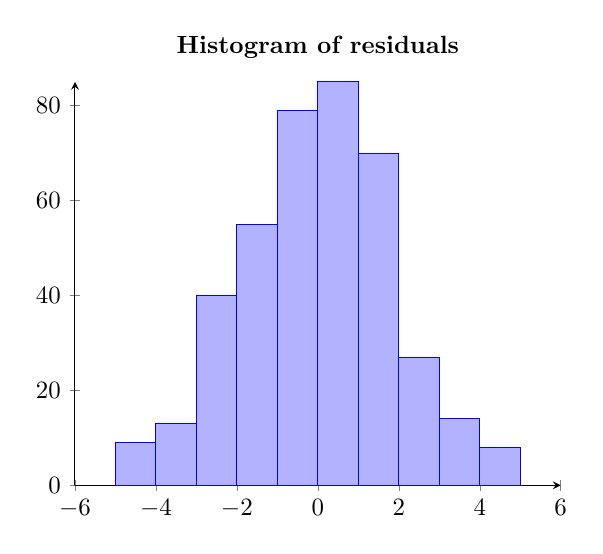
\begin{tikzpicture}[scale=0.9]
	\begin{axis}[
	ybar,
	ymin=0,
	axis y line=left,
	axis x line=bottom,
	domain=-6:-6,
	xmin=-6,
	xmax=6,
	title=\textbf{Histogram of residuals}
	]
	\addplot +[
	hist={
		bins=10,
		data min=-5,
		data max=5
	}   
	] table [y index=0] {
		dist
		-1.8970
		0.8230
		1.3540
		1.7155
		-1.3823
		0.8988
		0.2013
		1.6521
		1.0723
		1.7958
		-0.2639
		-0.2944
		2.0155
		-4.2473
		-1.0092
		-2.5412
		-0.7652
		1.2974
		1.6515
		-2.0299
		-0.9421
		0.2740
		-0.5837
		0.6036
		0.7999
		-1.8599
		-0.3537
		-4.2642
		2.2907
		-1.2582
		-2.4077
		-0.5079
		-2.8573
		-0.0417
		-1.1213
		4.3556
		2.2769
		-4.9938
		0.8827
		-2.7963
		-0.5101
		0.3288
		1.4955
		-0.5461
		3.1526
		-0.9619
		0.6550
		1.3295
		0.1704
		1.7619
		0.6464
		-1.5683
		-3.6107
		3.7172
		-1.2091
		0.2067
		1.1263
		0.2272
		-1.8095
		-0.9354
		-0.2498
		2.9579
		-1.7216
		1.5693
		0.6172
		-0.4677
		-2.1139
		-0.5683
		-0.1734
		-2.9388
		0.3844
		-1.6446
		-0.1885
		0.6724
		-1.8093
		-0.5765
		0.7001
		-3.6717
		2.0720
		4.8489
		1.9188
		-0.6315
		0.8572
		-2.0720
		3.7557
		1.8814
		1.5747
		-1.7517
		0.6399
		-1.1166
		-0.6229
		-1.1400
		-2.0515
		-1.8175
		-0.4198
		-3.3977
		1.2152
		-0.2356
		1.3983
		0.5393
		0.9886
		-2.9662
		-2.0405
		-0.8940
		0.2193
		2.2575
		-0.5799
		2.5231
		0.9508
		2.3482
		0.2539
		-1.3136
		-2.9628
		0.3110
		1.6371
		-0.5852
		-1.0816
		-0.6173
		-2.1932
		-0.9860
		-0.3615
		0.0917
		-0.1276
		1.2227
		0.2186
		3.6280
		0.6240
		3.6090
		-1.4462
		1.0531
		-0.5205
		1.2003
		1.1879
		-4.3720
		-2.6541
		-2.8820
		0.8037
		2.9404
		-0.6536
		1.6246
		1.0911
		-2.1033
		0.7949
		-1.5038
		3.0325
		-0.0651
		3.2720
		-0.8501
		1.1789
		-0.1256
		-4.0439
		-1.9643
		1.2250
		-0.1098
		-2.2375
		-1.2528
		0.4990
		-1.9860
		1.9499
		-1.2814
		3.6177
		-2.1597
		0.3984
		-3.0421
		-1.4473
		-1.1865
		0.8027
		1.8843
		0.6010
		-0.7461
		1.6310
		1.5978
		0.2404
		1.1425
		0.8256
		-1.9739
		1.5191
		-1.3144
		-1.2078
		0.3539
		-0.6150
		-0.2636
		1.1907
		2.0937
		-0.3959
		0.6554
		-0.4766
		0.4592
		0.8800
		-1.2337
		0.5497
		1.2022
		0.1846
		3.4597
		-1.2171
		-1.4741
		-3.4998
		1.8210
		1.7342
		-0.1598
		1.7970
		0.3674
		0.5816
		0.2259
		0.8799
		0.2033
		5.5747
		-2.3333
		-3.7086
		-2.2814
		-2.1867
		-0.8672
		-0.3369
		-0.4371
		1.0827
		0.7785
		1.5025
		3.5565
		2.4461
		-2.5665
		-4.6579
		1.8039
		-3.6713
		0.1335
		0.0710
		4.4543
		-0.1384
		-1.0146
		0.4716
		0.4916
		0.1401
		-1.2172
		-2.4452
		0.6330
		-2.6857
		-2.0644
		2.6624
		-0.8378
		-0.2806
		1.7996
		-0.6002
		2.0587
		-0.6901
		2.0256
		1.2587
		-0.4260
		-1.7314
		-2.0862
		-0.5401
		-0.8763
		-0.8173
		1.9671
		-0.5954
		2.2874
		-1.0632
		1.9451
		-1.0445
		0.3532
		1.9415
		-0.8279
		-0.8765
		4.0068
		1.9020
		-0.8640
		1.2979
		-0.7202
		1.4118
		2.8317
		-3.2090
		2.0577
		2.9159
		0.0949
		3.4925
		0.3108
		-2.4742
		-4.3870
		-0.6668
		1.4271
		0.6348
		0.8272
		-1.1542
		0.2880
		-3.2773
		-1.5202
		-1.6376
		1.0395
		-0.0283
		-2.3111
		-0.0190
		-1.3796
		-1.3334
		1.7283
		0.2268
		0.7967
		1.7679
		0.3605
		1.1017
		1.3659
		2.3412
		0.9517
		2.8245
		0.0452
		-0.0957
		3.4027
		-1.0194
		-0.0057
		1.8397
		0.2996
		2.8099
		2.0682
		0.5831
		-1.5554
		1.1334
		-2.7652
		0.4889
		1.6169
		0.4261
		1.7594
		4.0778
		1.8479
		0.5338
		1.2833
		0.8510
		-2.6294
		-0.8328
		2.4494
		-0.0872
		1.1648
		-2.0130
		0.1290
		1.2006
		-2.7230
		0.6952
		-0.3637
		-1.8791
		-0.0751
		-3.7926
		-4.2560
		-2.3538
		-1.9811
		-2.3461
		-3.4509
		0.5765
		-3.1884
		0.2204
		1.5741
		-0.0045
		0.1862
		-0.7563
		-2.9654
		-0.0876
		1.9217
		3.4765
		-0.8604
		-3.2546
		0.3327
		0.7525
		-0.4539
		-2.2978
		4.0487
		-4.7190
		-1.0199
		-2.6433
		-1.2723
		0.6357
		0.2761
		-1.4215
		1.5540
		1.2448
		1.2948
		-0.8513
		2.0972
		1.3214
		5.0175
		2.1269
		2.3138
		0.1060
		-2.5768
		-0.7424
		-1.5156
		-1.1279
		1.1103
		-1.1136
		-1.7902
		-0.8187
		-0.3218
		0.8187
		-1.9053
		0.6346
		0.1560
		2.6488
		-0.4263
		-0.2690
		-2.3427
		-2.7705
		0.6210
		-0.4990
		1.0075
		-1.7853
		3.8170
	};
	\end{axis}
	\end{tikzpicture}
	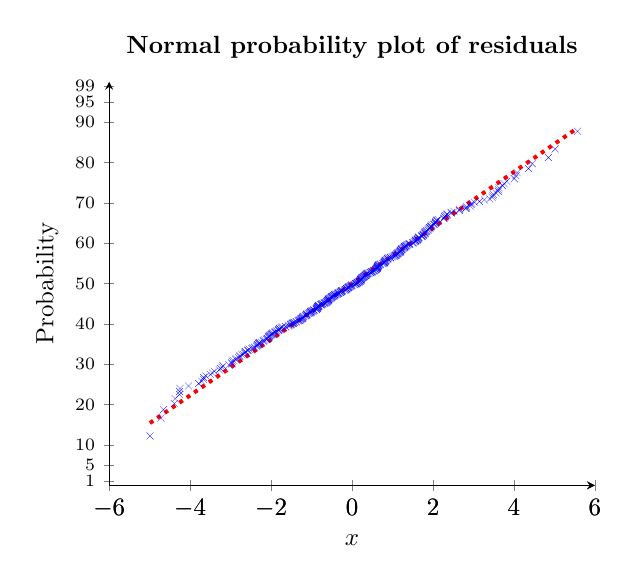
\begin{tikzpicture}[scale=0.9]
	\begin{axis}[
	xmin=-6, xmax=6, xlabel=$x$,
	ymin=-4, ymax=4, ylabel=$y$,
	samples=400,
	axis x line=bottom,
	axis y line=none,
	domain=-6:-6,
	title=\textbf{Normal probability plot of residuals}
	]
	\addplot[mark=x,blue, only marks, ultra thin] coordinates {
		(-4.99,-3.02)
		(-4.72,-2.67)
		(-4.66,-2.50)
		(-4.39,-2.38)
		(-4.37,-2.28)
		(-4.26,-2.20)
		(-4.26,-2.14)
		(-4.25,-2.08)
		(-4.04,-2.03)
		(-3.79,-1.98)
		(-3.71,-1.94)
		(-3.67,-1.90)
		(-3.67,-1.86)
		(-3.61,-1.83)
		(-3.50,-1.80)
		(-3.45,-1.77)
		(-3.40,-1.74)
		(-3.28,-1.71)
		(-3.25,-1.68)
		(-3.21,-1.66)
		(-3.19,-1.63)
		(-3.04,-1.61)
		(-2.97,-1.59)
		(-2.97,-1.57)
		(-2.96,-1.54)
		(-2.94,-1.52)
		(-2.88,-1.50)
		(-2.86,-1.49)
		(-2.80,-1.47)
		(-2.77,-1.45)
		(-2.77,-1.43)
		(-2.72,-1.41)
		(-2.69,-1.40)
		(-2.65,-1.38)
		(-2.64,-1.36)
		(-2.63,-1.35)
		(-2.58,-1.33)
		(-2.57,-1.32)
		(-2.54,-1.30)
		(-2.47,-1.29)
		(-2.45,-1.27)
		(-2.41,-1.26)
		(-2.35,-1.25)
		(-2.35,-1.23)
		(-2.34,-1.22)
		(-2.33,-1.21)
		(-2.31,-1.19)
		(-2.30,-1.18)
		(-2.28,-1.17)
		(-2.24,-1.16)
		(-2.19,-1.14)
		(-2.19,-1.13)
		(-2.16,-1.12)
		(-2.11,-1.11)
		(-2.10,-1.10)
		(-2.09,-1.09)
		(-2.07,-1.07)
		(-2.06,-1.06)
		(-2.05,-1.05)
		(-2.04,-1.04)
		(-2.03,-1.03)
		(-2.01,-1.02)
		(-1.99,-1.01)
		(-1.98,-1.00)
		(-1.97,-0.99)
		(-1.96,-0.98)
		(-1.91,-0.97)
		(-1.90,-0.96)
		(-1.88,-0.95)
		(-1.86,-0.94)
		(-1.82,-0.93)
		(-1.81,-0.92)
		(-1.81,-0.91)
		(-1.79,-0.90)
		(-1.79,-0.89)
		(-1.75,-0.88)
		(-1.73,-0.87)
		(-1.72,-0.86)
		(-1.64,-0.86)
		(-1.64,-0.85)
		(-1.57,-0.84)
		(-1.56,-0.83)
		(-1.52,-0.82)
		(-1.52,-0.81)
		(-1.50,-0.80)
		(-1.47,-0.79)
		(-1.45,-0.78)
		(-1.45,-0.78)
		(-1.42,-0.77)
		(-1.38,-0.76)
		(-1.38,-0.75)
		(-1.33,-0.74)
		(-1.31,-0.73)
		(-1.31,-0.73)
		(-1.28,-0.72)
		(-1.27,-0.71)
		(-1.26,-0.70)
		(-1.25,-0.69)
		(-1.23,-0.69)
		(-1.22,-0.68)
		(-1.22,-0.67)
		(-1.21,-0.66)
		(-1.21,-0.65)
		(-1.19,-0.65)
		(-1.15,-0.64)
		(-1.14,-0.63)
		(-1.13,-0.62)
		(-1.12,-0.62)
		(-1.12,-0.61)
		(-1.11,-0.60)
		(-1.08,-0.59)
		(-1.06,-0.59)
		(-1.04,-0.58)
		(-1.02,-0.57)
		(-1.02,-0.56)
		(-1.01,-0.56)
		(-1.01,-0.55)
		(-0.99,-0.54)
		(-0.96,-0.54)
		(-0.94,-0.53)
		(-0.94,-0.52)
		(-0.89,-0.51)
		(-0.88,-0.51)
		(-0.88,-0.50)
		(-0.87,-0.49)
		(-0.86,-0.49)
		(-0.86,-0.48)
		(-0.85,-0.47)
		(-0.85,-0.46)
		(-0.84,-0.46)
		(-0.83,-0.45)
		(-0.83,-0.44)
		(-0.82,-0.44)
		(-0.82,-0.43)
		(-0.77,-0.42)
		(-0.76,-0.42)
		(-0.75,-0.41)
		(-0.74,-0.40)
		(-0.72,-0.40)
		(-0.69,-0.39)
		(-0.67,-0.38)
		(-0.65,-0.38)
		(-0.63,-0.37)
		(-0.62,-0.36)
		(-0.62,-0.36)
		(-0.62,-0.35)
		(-0.60,-0.34)
		(-0.60,-0.34)
		(-0.59,-0.33)
		(-0.58,-0.32)
		(-0.58,-0.32)
		(-0.58,-0.31)
		(-0.57,-0.30)
		(-0.55,-0.30)
		(-0.54,-0.29)
		(-0.52,-0.28)
		(-0.51,-0.28)
		(-0.51,-0.27)
		(-0.50,-0.26)
		(-0.48,-0.26)
		(-0.47,-0.25)
		(-0.45,-0.24)
		(-0.44,-0.24)
		(-0.43,-0.23)
		(-0.43,-0.22)
		(-0.42,-0.22)
		(-0.40,-0.21)
		(-0.36,-0.21)
		(-0.36,-0.20)
		(-0.35,-0.19)
		(-0.34,-0.19)
		(-0.32,-0.18)
		(-0.29,-0.17)
		(-0.28,-0.17)
		(-0.27,-0.16)
		(-0.26,-0.15)
		(-0.26,-0.15)
		(-0.25,-0.14)
		(-0.24,-0.14)
		(-0.19,-0.13)
		(-0.17,-0.12)
		(-0.16,-0.12)
		(-0.14,-0.11)
		(-0.13,-0.10)
		(-0.13,-0.10)
		(-0.11,-0.09)
		(-0.10,-0.08)
		(-0.09,-0.08)
		(-0.09,-0.07)
		(-0.08,-0.07)
		(-0.07,-0.06)
		(-0.04,-0.05)
		(-0.03,-0.05)
		(-0.02,-0.04)
		(-0.01,-0.03)
		(-0.00,-0.03)
		(0.05,-0.02)
		(0.07,-0.02)
		(0.09,-0.01)
		(0.09,-0.00)
		(0.11,0.00)
		(0.13,0.01)
		(0.13,0.02)
		(0.14,0.02)
		(0.16,0.03)
		(0.17,0.03)
		(0.18,0.04)
		(0.19,0.05)
		(0.20,0.05)
		(0.20,0.06)
		(0.21,0.07)
		(0.22,0.07)
		(0.22,0.08)
		(0.22,0.08)
		(0.23,0.09)
		(0.23,0.10)
		(0.23,0.10)
		(0.24,0.11)
		(0.25,0.12)
		(0.27,0.12)
		(0.28,0.13)
		(0.29,0.14)
		(0.30,0.14)
		(0.31,0.15)
		(0.31,0.15)
		(0.33,0.16)
		(0.33,0.17)
		(0.35,0.17)
		(0.35,0.18)
		(0.36,0.19)
		(0.37,0.19)
		(0.38,0.20)
		(0.40,0.21)
		(0.43,0.21)
		(0.46,0.22)
		(0.47,0.22)
		(0.49,0.23)
		(0.49,0.24)
		(0.50,0.24)
		(0.53,0.25)
		(0.54,0.26)
		(0.55,0.26)
		(0.58,0.27)
		(0.58,0.28)
		(0.58,0.28)
		(0.60,0.29)
		(0.60,0.30)
		(0.62,0.30)
		(0.62,0.31)
		(0.62,0.32)
		(0.63,0.32)
		(0.63,0.33)
		(0.63,0.34)
		(0.64,0.34)
		(0.64,0.35)
		(0.65,0.36)
		(0.66,0.36)
		(0.66,0.37)
		(0.67,0.38)
		(0.70,0.38)
		(0.70,0.39)
		(0.75,0.40)
		(0.78,0.40)
		(0.79,0.41)
		(0.80,0.42)
		(0.80,0.42)
		(0.80,0.43)
		(0.80,0.44)
		(0.82,0.44)
		(0.82,0.45)
		(0.83,0.46)
		(0.83,0.46)
		(0.85,0.47)
		(0.86,0.48)
		(0.88,0.49)
		(0.88,0.49)
		(0.88,0.50)
		(0.90,0.51)
		(0.95,0.51)
		(0.95,0.52)
		(0.99,0.53)
		(1.01,0.54)
		(1.04,0.54)
		(1.05,0.55)
		(1.07,0.56)
		(1.08,0.56)
		(1.09,0.57)
		(1.10,0.58)
		(1.11,0.59)
		(1.13,0.59)
		(1.13,0.60)
		(1.14,0.61)
		(1.16,0.62)
		(1.18,0.62)
		(1.19,0.63)
		(1.19,0.64)
		(1.20,0.65)
		(1.20,0.65)
		(1.20,0.66)
		(1.22,0.67)
		(1.22,0.68)
		(1.23,0.69)
		(1.24,0.69)
		(1.26,0.70)
		(1.28,0.71)
		(1.29,0.72)
		(1.30,0.73)
		(1.30,0.73)
		(1.32,0.74)
		(1.33,0.75)
		(1.35,0.76)
		(1.37,0.77)
		(1.40,0.78)
		(1.41,0.78)
		(1.43,0.79)
		(1.50,0.80)
		(1.50,0.81)
		(1.52,0.82)
		(1.55,0.83)
		(1.57,0.84)
		(1.57,0.85)
		(1.57,0.86)
		(1.60,0.86)
		(1.62,0.87)
		(1.62,0.88)
		(1.63,0.89)
		(1.64,0.90)
		(1.65,0.91)
		(1.65,0.92)
		(1.72,0.93)
		(1.73,0.94)
		(1.73,0.95)
		(1.76,0.96)
		(1.76,0.97)
		(1.77,0.98)
		(1.80,0.99)
		(1.80,1.00)
		(1.80,1.01)
		(1.80,1.02)
		(1.82,1.03)
		(1.84,1.04)
		(1.85,1.05)
		(1.88,1.06)
		(1.88,1.07)
		(1.90,1.09)
		(1.92,1.10)
		(1.92,1.11)
		(1.94,1.12)
		(1.95,1.13)
		(1.95,1.14)
		(1.97,1.16)
		(2.02,1.17)
		(2.03,1.18)
		(2.06,1.19)
		(2.06,1.21)
		(2.07,1.22)
		(2.07,1.23)
		(2.09,1.25)
		(2.10,1.26)
		(2.13,1.27)
		(2.26,1.29)
		(2.28,1.30)
		(2.29,1.32)
		(2.29,1.33)
		(2.31,1.35)
		(2.34,1.36)
		(2.35,1.38)
		(2.45,1.40)
		(2.45,1.41)
		(2.52,1.43)
		(2.65,1.45)
		(2.66,1.47)
		(2.81,1.49)
		(2.82,1.50)
		(2.83,1.52)
		(2.92,1.54)
		(2.94,1.57)
		(2.96,1.59)
		(3.03,1.61)
		(3.15,1.63)
		(3.27,1.66)
		(3.40,1.68)
		(3.46,1.71)
		(3.48,1.74)
		(3.49,1.77)
		(3.56,1.80)
		(3.61,1.83)
		(3.62,1.86)
		(3.63,1.90)
		(3.72,1.94)
		(3.76,1.98)
		(3.82,2.03)
		(4.01,2.08)
		(4.05,2.14)
		(4.08,2.20)
		(4.36,2.28)
		(4.45,2.38)
		(4.85,2.50)
		(5.02,2.67)
		(5.57,3.02)
	};
	\addplot[dotted,red,ultra thick] coordinates {
		(-4.9938,-2.7658)
		(5.5747,3.0865)
	};
	\end{axis}
	\begin{axis}[
	xmin=-6,
	xmax=6,
	ymin=0,
	ymax=100,
	ylabel=Probability,
	axis y line=left,
	axis x line=bottom,
	yticklabel style={font=\scriptsize},
	ytick={1,5,10,20,30,40,50,60,70,80,90,95,99},
	]
	\end{axis}
	\end{tikzpicture}
\end{center}
\input{./TeX_files/materials/perfect_residuals_2}

The following residual plots gone wrong. Note that these plots are not all from the same data.

\begin{center}
	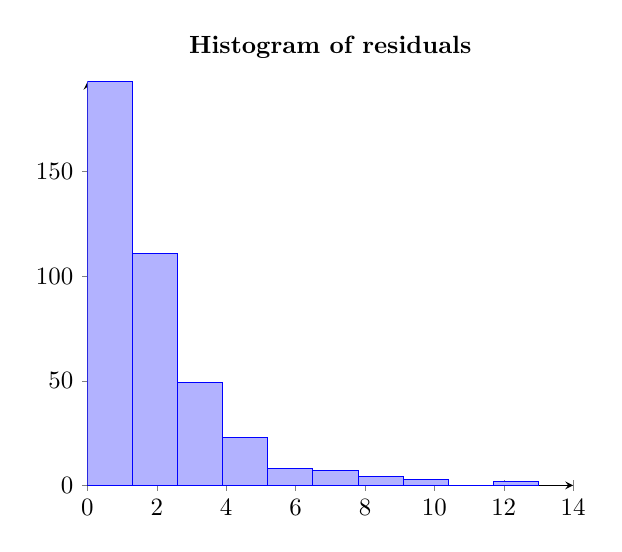
\begin{tikzpicture}[scale=0.9]
	\begin{axis}[
	ybar,
	ymin=0,
	axis y line=left,
	axis x line=bottom,
	domain=0:14,
	xmin=0,
	xmax=14,
	title=\textbf{Histogram of residuals}
	]
	\addplot +[
	hist={
		bins=10,
		data min=0,
		data max=13
	}   
	] table [y index=0] {
		dist
		3.9882
		0.8133
		0.3716
		0.7902
		3.9400
		1.9414
		0.7761
		1.3236
		0.0444
		2.6356
		0.2856
		1.9683
		3.9810
		4.9853
		0.6054
		1.9774
		1.9325
		2.3935
		2.4448
		2.6956
		1.5380
		0.0244
		1.9086
		0.1169
		3.5795
		0.1559
		0.5638
		0.3096
		1.0137
		4.4630
		1.5728
		0.8475
		5.7108
		7.7016
		2.4771
		0.1420
		1.3310
		0.2664
		1.9452
		0.2454
		1.2518
		0.2272
		4.5507
		3.1019
		0.7088
		2.0358
		13.1487
		1.9126
		2.2780
		1.8661
		3.4157
		3.1272
		1.0427
		1.0402
		3.5151
		0.1387
		5.7571
		3.2017
		1.3536
		0.5509
		3.8476
		0.1428
		1.7257
		5.7471
		0.7885
		2.5473
		0.4967
		0.0757
		0.7472
		1.3926
		4.6246
		2.4913
		1.2394
		8.9606
		2.5257
		1.0567
		3.5200
		3.5428
		0.7821
		1.1257
		1.1896
		0.0662
		0.9291
		2.2506
		1.3040
		0.2902
		0.0118
		0.3523
		2.1146
		0.5769
		0.1250
		0.8067
		1.4629
		2.5024
		1.0379
		2.1789
		0.0826
		1.6326
		0.0775
		0.7820
		0.6961
		0.0865
		0.1240
		0.3636
		3.7255
		0.3716
		1.5351
		2.4167
		1.2952
		0.3687
		1.2356
		2.6954
		2.0767
		3.3561
		2.0959
		3.3244
		0.3590
		1.9134
		9.3130
		2.3487
		0.3565
		2.5364
		0.4935
		1.2641
		3.7427
		1.2877
		2.5229
		0.6713
		0.6174
		1.5986
		3.4066
		3.9970
		2.5982
		0.9062
		0.4309
		0.8073
		2.4994
		3.8976
		2.8059
		0.7366
		5.2692
		1.3917
		0.0282
		0.1999
		1.1060
		0.5318
		0.5840
		0.7267
		0.7792
		2.5289
		1.0830
		0.9597
		0.4110
		8.2720
		3.0803
		0.0244
		0.4034
		0.9175
		0.7650
		0.4258
		2.5483
		0.8160
		7.0587
		1.2162
		1.2736
		0.2713
		3.3468
		0.1420
		0.0479
		2.2100
		0.9441
		1.2809
		1.5571
		2.0513
		2.1916
		4.9731
		1.8812
		2.8597
		1.4420
		0.7131
		3.9716
		0.3812
		0.1450
		0.3757
		1.4474
		0.8317
		1.5688
		1.7423
		6.7454
		0.1519
		6.2755
		1.4844
		1.9051
		1.2545
		0.0037
		0.2052
		8.4323
		0.4956
		1.4460
		1.8821
		0.3894
		0.2684
		0.0033
		3.2627
		0.2786
		2.3586
		1.7772
		0.4058
		1.9980
		1.7056
		4.7890
		0.8084
		0.6258
		2.4025
		2.1694
		0.6176
		0.0293
		0.7169
		4.8174
		1.5069
		0.9071
		1.2877
		3.9132
		2.5782
		0.0260
		0.4588
		0.1380
		2.1090
		3.1296
		0.7703
		2.0689
		1.6494
		0.1913
		0.3640
		1.8761
		0.6185
		2.4712
		2.4611
		2.4294
		7.3904
		0.1715
		0.7537
		2.9025
		1.3969
		0.4700
		1.9339
		3.0412
		0.6496
		0.5154
		0.7326
		0.9571
		0.5428
		1.3409
		2.2209
		13.2241
		1.0872
		3.5224
		3.2705
		3.7900
		1.3647
		8.1041
		1.5049
		6.1549
		1.6317
		3.6212
		1.1169
		0.4010
		4.9222
		2.9148
		2.8045
		2.0886
		1.7877
		4.3389
		1.7968
		0.7833
		1.2212
		2.0593
		0.8262
		0.7751
		4.0566
		1.6437
		0.1297
		1.1235
		1.0976
		0.5368
		2.7971
		0.7310
		2.4425
		1.1218
		0.9089
		1.8381
		2.7815
		0.1337
		1.6019
		1.2630
		0.9088
		0.8066
		1.6465
		3.5091
		0.7295
		0.1561
		1.9852
		0.8964
		0.2338
		1.4557
		0.9246
		1.5314
		4.4296
		4.3587
		4.4532
		1.6161
		0.1262
		0.9120
		0.1459
		5.5332
		2.3622
		0.1031
		9.1388
		3.5696
		0.5614
		0.3635
		1.0022
		1.3159
		0.1177
		0.5990
		0.7103
		0.5895
		0.2697
		0.0731
		0.0365
		0.1697
		2.5212
		5.6732
		0.3945
		3.4349
		6.7087
		0.5193
		1.2304
		2.2080
		1.0956
		0.3145
		0.8852
		1.7345
		1.2106
		3.4042
		2.8855
		3.1655
		2.6966
		0.1182
		0.8877
		0.3749
		1.8896
		3.5627
		0.6019
		0.2721
		2.0683
		3.4427
		0.0072
		0.0835
		3.7158
		0.1474
		1.7133
		3.0004
		3.9844
		2.6928
		1.2159
		4.9970
		1.0279
		7.0681
		1.5753
		2.2022
		0.1160
		2.3874
		1.6962
		0.8279
		1.9294
		3.9877
		4.6738
		2.3738
		0.3875
		0.9328
		3.1604
		0.0400
		1.6521
		0.3602
		1.2354
		7.3676
		9.9745
		0.4814
		1.6086
		2.4845
		0.2943
		0.8425
		2.5127
		0.8784
		2.6668
		3.4885
		1.9960
		1.2415
		0.1529
	};
	\end{axis}
	\end{tikzpicture}
	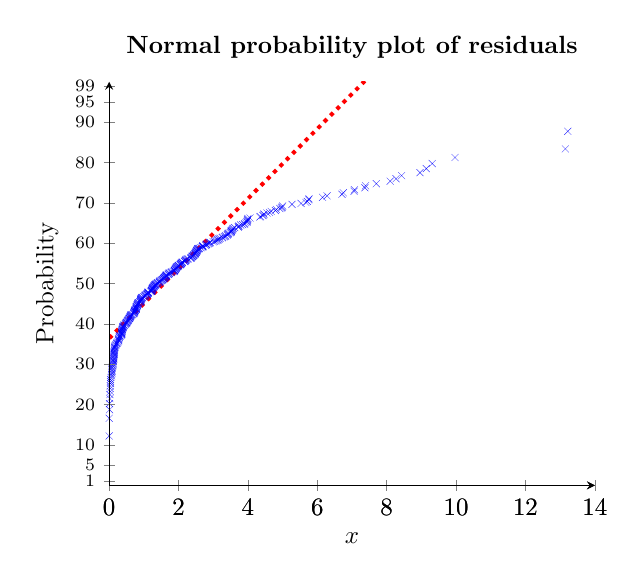
\begin{tikzpicture}[scale=0.9]
	\begin{axis}[
	xmin=0, xmax=14, xlabel=$x$,
	ymin=-4, ymax=4, ylabel=$y$,
	samples=400,
	axis x line=bottom,
	axis y line=none,
	domain=-6:-6,
	title=\textbf{Normal probability plot of residuals}
	]
	\addplot[mark=x,blue, only marks, ultra thin] coordinates {
		(0.00,-3.02)
		(0.00,-2.67)
		(0.01,-2.50)
		(0.01,-2.38)
		(0.02,-2.28)
		(0.02,-2.20)
		(0.03,-2.14)
		(0.03,-2.08)
		(0.03,-2.03)
		(0.04,-1.98)
		(0.04,-1.94)
		(0.04,-1.90)
		(0.05,-1.86)
		(0.07,-1.83)
		(0.07,-1.80)
		(0.08,-1.77)
		(0.08,-1.74)
		(0.08,-1.71)
		(0.08,-1.68)
		(0.09,-1.66)
		(0.10,-1.63)
		(0.12,-1.61)
		(0.12,-1.59)
		(0.12,-1.57)
		(0.12,-1.54)
		(0.12,-1.52)
		(0.13,-1.50)
		(0.13,-1.49)
		(0.13,-1.47)
		(0.13,-1.45)
		(0.14,-1.43)
		(0.14,-1.41)
		(0.14,-1.40)
		(0.14,-1.38)
		(0.14,-1.36)
		(0.15,-1.35)
		(0.15,-1.33)
		(0.15,-1.32)
		(0.15,-1.30)
		(0.15,-1.29)
		(0.16,-1.27)
		(0.16,-1.26)
		(0.17,-1.25)
		(0.17,-1.23)
		(0.19,-1.22)
		(0.20,-1.21)
		(0.21,-1.19)
		(0.23,-1.18)
		(0.23,-1.17)
		(0.25,-1.16)
		(0.27,-1.14)
		(0.27,-1.13)
		(0.27,-1.12)
		(0.27,-1.11)
		(0.27,-1.10)
		(0.28,-1.09)
		(0.29,-1.07)
		(0.29,-1.06)
		(0.29,-1.05)
		(0.31,-1.04)
		(0.31,-1.03)
		(0.35,-1.02)
		(0.36,-1.01)
		(0.36,-1.00)
		(0.36,-0.99)
		(0.36,-0.98)
		(0.36,-0.97)
		(0.36,-0.96)
		(0.37,-0.95)
		(0.37,-0.94)
		(0.37,-0.93)
		(0.37,-0.92)
		(0.38,-0.91)
		(0.38,-0.90)
		(0.39,-0.89)
		(0.39,-0.88)
		(0.39,-0.87)
		(0.40,-0.86)
		(0.40,-0.86)
		(0.41,-0.85)
		(0.41,-0.84)
		(0.43,-0.83)
		(0.43,-0.82)
		(0.46,-0.81)
		(0.47,-0.80)
		(0.48,-0.79)
		(0.49,-0.78)
		(0.50,-0.78)
		(0.50,-0.77)
		(0.52,-0.76)
		(0.52,-0.75)
		(0.53,-0.74)
		(0.54,-0.73)
		(0.54,-0.73)
		(0.55,-0.72)
		(0.56,-0.71)
		(0.56,-0.70)
		(0.58,-0.69)
		(0.58,-0.69)
		(0.59,-0.68)
		(0.60,-0.67)
		(0.60,-0.66)
		(0.61,-0.65)
		(0.62,-0.65)
		(0.62,-0.64)
		(0.62,-0.63)
		(0.63,-0.62)
		(0.65,-0.62)
		(0.67,-0.61)
		(0.70,-0.60)
		(0.71,-0.59)
		(0.71,-0.59)
		(0.71,-0.58)
		(0.72,-0.57)
		(0.73,-0.56)
		(0.73,-0.56)
		(0.73,-0.55)
		(0.73,-0.54)
		(0.74,-0.54)
		(0.75,-0.53)
		(0.75,-0.52)
		(0.77,-0.51)
		(0.77,-0.51)
		(0.78,-0.50)
		(0.78,-0.49)
		(0.78,-0.49)
		(0.78,-0.48)
		(0.78,-0.47)
		(0.78,-0.46)
		(0.79,-0.46)
		(0.79,-0.45)
		(0.81,-0.44)
		(0.81,-0.44)
		(0.81,-0.43)
		(0.81,-0.42)
		(0.81,-0.42)
		(0.82,-0.41)
		(0.83,-0.40)
		(0.83,-0.40)
		(0.83,-0.39)
		(0.84,-0.38)
		(0.85,-0.38)
		(0.88,-0.37)
		(0.89,-0.36)
		(0.89,-0.36)
		(0.90,-0.35)
		(0.91,-0.34)
		(0.91,-0.34)
		(0.91,-0.33)
		(0.91,-0.32)
		(0.91,-0.32)
		(0.92,-0.31)
		(0.92,-0.30)
		(0.93,-0.30)
		(0.93,-0.29)
		(0.94,-0.28)
		(0.96,-0.28)
		(0.96,-0.27)
		(1.00,-0.26)
		(1.01,-0.26)
		(1.03,-0.25)
		(1.04,-0.24)
		(1.04,-0.24)
		(1.04,-0.23)
		(1.06,-0.22)
		(1.08,-0.22)
		(1.09,-0.21)
		(1.10,-0.21)
		(1.10,-0.20)
		(1.11,-0.19)
		(1.12,-0.19)
		(1.12,-0.18)
		(1.12,-0.17)
		(1.13,-0.17)
		(1.19,-0.16)
		(1.21,-0.15)
		(1.22,-0.15)
		(1.22,-0.14)
		(1.22,-0.14)
		(1.23,-0.13)
		(1.24,-0.12)
		(1.24,-0.12)
		(1.24,-0.11)
		(1.24,-0.10)
		(1.25,-0.10)
		(1.25,-0.09)
		(1.26,-0.08)
		(1.26,-0.08)
		(1.27,-0.07)
		(1.28,-0.07)
		(1.29,-0.06)
		(1.29,-0.05)
		(1.30,-0.05)
		(1.30,-0.04)
		(1.32,-0.03)
		(1.32,-0.03)
		(1.33,-0.02)
		(1.34,-0.02)
		(1.35,-0.01)
		(1.36,-0.00)
		(1.39,0.00)
		(1.39,0.01)
		(1.40,0.02)
		(1.44,0.02)
		(1.45,0.03)
		(1.45,0.03)
		(1.46,0.04)
		(1.46,0.05)
		(1.48,0.05)
		(1.50,0.06)
		(1.51,0.07)
		(1.53,0.07)
		(1.54,0.08)
		(1.54,0.08)
		(1.56,0.09)
		(1.57,0.10)
		(1.57,0.10)
		(1.58,0.11)
		(1.60,0.12)
		(1.60,0.12)
		(1.61,0.13)
		(1.62,0.14)
		(1.63,0.14)
		(1.63,0.15)
		(1.64,0.15)
		(1.65,0.16)
		(1.65,0.17)
		(1.65,0.17)
		(1.70,0.18)
		(1.71,0.19)
		(1.71,0.19)
		(1.73,0.20)
		(1.73,0.21)
		(1.74,0.21)
		(1.78,0.22)
		(1.79,0.22)
		(1.80,0.23)
		(1.84,0.24)
		(1.87,0.24)
		(1.88,0.25)
		(1.88,0.26)
		(1.88,0.26)
		(1.89,0.27)
		(1.91,0.28)
		(1.91,0.28)
		(1.91,0.29)
		(1.91,0.30)
		(1.93,0.30)
		(1.93,0.31)
		(1.93,0.32)
		(1.94,0.32)
		(1.95,0.33)
		(1.97,0.34)
		(1.98,0.34)
		(1.99,0.35)
		(2.00,0.36)
		(2.00,0.36)
		(2.04,0.37)
		(2.05,0.38)
		(2.06,0.38)
		(2.07,0.39)
		(2.07,0.40)
		(2.08,0.40)
		(2.09,0.41)
		(2.10,0.42)
		(2.11,0.42)
		(2.11,0.43)
		(2.17,0.44)
		(2.18,0.44)
		(2.19,0.45)
		(2.20,0.46)
		(2.21,0.46)
		(2.21,0.47)
		(2.22,0.48)
		(2.25,0.49)
		(2.28,0.49)
		(2.35,0.50)
		(2.36,0.51)
		(2.36,0.51)
		(2.37,0.52)
		(2.39,0.53)
		(2.39,0.54)
		(2.40,0.54)
		(2.42,0.55)
		(2.43,0.56)
		(2.44,0.56)
		(2.44,0.57)
		(2.46,0.58)
		(2.47,0.59)
		(2.48,0.59)
		(2.48,0.60)
		(2.49,0.61)
		(2.50,0.62)
		(2.50,0.62)
		(2.51,0.63)
		(2.52,0.64)
		(2.52,0.65)
		(2.53,0.65)
		(2.53,0.66)
		(2.54,0.67)
		(2.55,0.68)
		(2.55,0.69)
		(2.58,0.69)
		(2.60,0.70)
		(2.64,0.71)
		(2.67,0.72)
		(2.69,0.73)
		(2.70,0.73)
		(2.70,0.74)
		(2.70,0.75)
		(2.78,0.76)
		(2.80,0.77)
		(2.80,0.78)
		(2.81,0.78)
		(2.86,0.79)
		(2.89,0.80)
		(2.90,0.81)
		(2.91,0.82)
		(3.00,0.83)
		(3.04,0.84)
		(3.08,0.85)
		(3.10,0.86)
		(3.13,0.86)
		(3.13,0.87)
		(3.16,0.88)
		(3.17,0.89)
		(3.20,0.90)
		(3.26,0.91)
		(3.27,0.92)
		(3.32,0.93)
		(3.35,0.94)
		(3.36,0.95)
		(3.40,0.96)
		(3.41,0.97)
		(3.42,0.98)
		(3.43,0.99)
		(3.44,1.00)
		(3.49,1.01)
		(3.51,1.02)
		(3.52,1.03)
		(3.52,1.04)
		(3.52,1.05)
		(3.54,1.06)
		(3.56,1.07)
		(3.57,1.09)
		(3.58,1.10)
		(3.62,1.11)
		(3.72,1.12)
		(3.73,1.13)
		(3.74,1.14)
		(3.79,1.16)
		(3.85,1.17)
		(3.90,1.18)
		(3.91,1.19)
		(3.94,1.21)
		(3.97,1.22)
		(3.98,1.23)
		(3.98,1.25)
		(3.99,1.26)
		(3.99,1.27)
		(4.00,1.29)
		(4.06,1.30)
		(4.34,1.32)
		(4.36,1.33)
		(4.43,1.35)
		(4.45,1.36)
		(4.46,1.38)
		(4.55,1.40)
		(4.62,1.41)
		(4.67,1.43)
		(4.79,1.45)
		(4.82,1.47)
		(4.92,1.49)
		(4.97,1.50)
		(4.99,1.52)
		(5.00,1.54)
		(5.27,1.57)
		(5.53,1.59)
		(5.67,1.61)
		(5.71,1.63)
		(5.75,1.66)
		(5.76,1.68)
		(6.15,1.71)
		(6.28,1.74)
		(6.71,1.77)
		(6.75,1.80)
		(7.06,1.83)
		(7.07,1.86)
		(7.37,1.90)
		(7.39,1.94)
		(7.70,1.98)
		(8.10,2.03)
		(8.27,2.08)
		(8.43,2.14)
		(8.96,2.20)
		(9.14,2.28)
		(9.31,2.38)
		(9.97,2.50)
		(13.15,2.67)
		(13.22,3.02)
	};
	\addplot[dotted,red,ultra thick] coordinates {
		(0.0033,-1.0838)
		(13.2241,8.0734)
	};
	\end{axis}
	\begin{axis}[
	xmin=0,
	xmax=14,
	ymin=0,
	ymax=100,
	ylabel=Probability,
	axis y line=left,
	axis x line=bottom,
	yticklabel style={font=\scriptsize},
	ytick={1,5,10,20,30,40,50,60,70,80,90,95,99},
	]
	\end{axis}
	\end{tikzpicture}
\end{center}
\begin{center}
	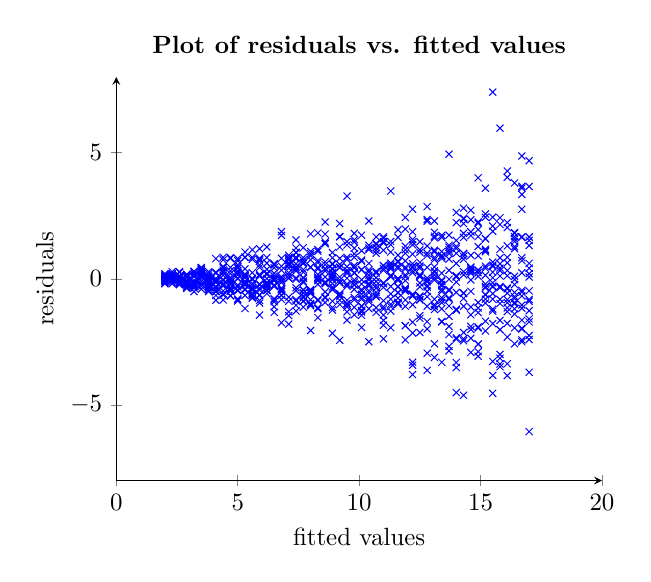
\begin{tikzpicture}[scale=0.9]
	\begin{axis}[
		xmin=0, xmax=20, xlabel=fitted values,
		ymin=-8, ymax=8, ylabel=residuals,
		samples=400,
		axis x line=bottom,
		axis y line=left,
		domain=0:20,
		title=\textbf{Plot of residuals vs. fitted values}
	]
		\addplot[mark=x,blue, only marks] coordinates {
			(2.00,0.06)
			(2.00,-0.09)
			(2.00,-0.17)
			(2.00,-0.08)
			(2.00,0.15)
			(2.00,0.05)
			(2.00,-0.11)
			(2.00,0.13)
			(2.00,-0.08)
			(2.00,-0.00)
			(2.00,-0.07)
			(2.00,-0.00)
			(2.00,-0.07)
			(2.00,-0.07)
			(2.00,-0.07)
			(2.00,0.20)
			(2.00,-0.20)
			(2.00,0.10)
			(2.00,-0.05)
			(2.00,0.06)
			(2.30,0.14)
			(2.30,-0.20)
			(2.30,0.10)
			(2.30,-0.04)
			(2.30,-0.14)
			(2.30,-0.00)
			(2.30,-0.01)
			(2.30,0.04)
			(2.30,0.06)
			(2.30,-0.04)
			(2.30,0.10)
			(2.30,0.04)
			(2.30,0.18)
			(2.30,0.20)
			(2.30,-0.07)
			(2.30,-0.04)
			(2.30,0.15)
			(2.30,0.28)
			(2.30,0.18)
			(2.30,-0.00)
			(2.60,0.04)
			(2.60,0.28)
			(2.60,-0.20)
			(2.60,-0.04)
			(2.60,-0.14)
			(2.60,0.25)
			(2.60,-0.22)
			(2.60,-0.09)
			(2.60,0.01)
			(2.60,0.06)
			(2.60,-0.07)
			(2.60,-0.18)
			(2.60,-0.06)
			(2.60,-0.06)
			(2.60,-0.21)
			(2.60,-0.24)
			(2.60,0.04)
			(2.60,0.12)
			(2.60,0.09)
			(2.60,-0.00)
			(2.90,-0.13)
			(2.90,-0.35)
			(2.90,-0.22)
			(2.90,-0.13)
			(2.90,-0.06)
			(2.90,0.05)
			(2.90,0.05)
			(2.90,0.18)
			(2.90,0.07)
			(2.90,-0.30)
			(2.90,0.17)
			(2.90,-0.23)
			(2.90,-0.10)
			(2.90,-0.16)
			(2.90,0.13)
			(2.90,-0.38)
			(2.90,0.12)
			(2.90,-0.16)
			(2.90,-0.19)
			(2.90,-0.29)
			(3.20,-0.22)
			(3.20,-0.32)
			(3.20,-0.24)
			(3.20,0.29)
			(3.20,-0.06)
			(3.20,-0.28)
			(3.20,0.29)
			(3.20,0.14)
			(3.20,0.08)
			(3.20,-0.15)
			(3.20,0.16)
			(3.20,-0.17)
			(3.20,-0.21)
			(3.20,-0.16)
			(3.20,-0.13)
			(3.20,0.12)
			(3.20,0.22)
			(3.20,-0.51)
			(3.20,-0.13)
			(3.20,-0.37)
			(3.50,0.34)
			(3.50,0.45)
			(3.50,-0.20)
			(3.50,0.24)
			(3.50,0.15)
			(3.50,0.10)
			(3.50,0.26)
			(3.50,0.21)
			(3.50,0.06)
			(3.50,-0.22)
			(3.50,0.43)
			(3.50,-0.30)
			(3.50,-0.03)
			(3.50,-0.11)
			(3.50,0.29)
			(3.50,0.34)
			(3.50,0.37)
			(3.50,0.41)
			(3.50,-0.41)
			(3.50,0.10)
			(3.80,0.00)
			(3.80,-0.21)
			(3.80,0.06)
			(3.80,-0.10)
			(3.80,-0.41)
			(3.80,-0.26)
			(3.80,-0.32)
			(3.80,-0.30)
			(3.80,-0.04)
			(3.80,0.06)
			(3.80,-0.32)
			(3.80,-0.51)
			(3.80,-0.35)
			(3.80,0.20)
			(3.80,0.28)
			(3.80,-0.47)
			(3.80,0.11)
			(3.80,-0.15)
			(3.80,-0.31)
			(3.80,0.09)
			(4.10,-0.51)
			(4.10,-0.51)
			(4.10,-0.14)
			(4.10,-0.85)
			(4.10,-0.30)
			(4.10,-0.49)
			(4.10,-0.66)
			(4.10,-0.33)
			(4.10,0.01)
			(4.10,-0.12)
			(4.10,0.80)
			(4.10,-0.07)
			(4.10,-0.33)
			(4.10,0.26)
			(4.10,0.22)
			(4.10,-0.35)
			(4.10,-0.05)
			(4.10,-0.43)
			(4.10,-0.14)
			(4.10,-0.12)
			(4.40,0.85)
			(4.40,0.27)
			(4.40,-0.48)
			(4.40,-0.59)
			(4.40,-0.29)
			(4.40,0.14)
			(4.40,0.75)
			(4.40,-0.25)
			(4.40,-0.07)
			(4.40,-0.64)
			(4.40,0.49)
			(4.40,0.24)
			(4.40,0.35)
			(4.40,0.29)
			(4.40,-0.84)
			(4.40,0.45)
			(4.40,-0.03)
			(4.40,-0.25)
			(4.40,-0.19)
			(4.40,0.44)
			(4.70,0.84)
			(4.70,0.45)
			(4.70,0.80)
			(4.70,-0.24)
			(4.70,-0.68)
			(4.70,-0.17)
			(4.70,-0.48)
			(4.70,-0.49)
			(4.70,-0.17)
			(4.70,-0.66)
			(4.70,-0.40)
			(4.70,-0.05)
			(4.70,0.05)
			(4.70,-0.35)
			(4.70,-0.12)
			(4.70,-0.01)
			(4.70,-0.16)
			(4.70,0.31)
			(4.70,-0.40)
			(4.70,0.20)
			(5.00,0.72)
			(5.00,0.80)
			(5.00,-0.25)
			(5.00,0.24)
			(5.00,-0.47)
			(5.00,0.22)
			(5.00,-0.80)
			(5.00,-0.83)
			(5.00,-0.44)
			(5.00,-0.88)
			(5.00,0.24)
			(5.00,0.03)
			(5.00,0.47)
			(5.00,0.15)
			(5.00,0.31)
			(5.00,-0.47)
			(5.00,0.42)
			(5.00,-0.01)
			(5.00,-0.32)
			(5.00,0.55)
			(5.30,0.39)
			(5.30,-0.10)
			(5.30,0.14)
			(5.30,-0.19)
			(5.30,-0.44)
			(5.30,0.11)
			(5.30,-0.14)
			(5.30,-0.20)
			(5.30,0.19)
			(5.30,-0.25)
			(5.30,-0.17)
			(5.30,0.86)
			(5.30,-1.18)
			(5.30,-0.40)
			(5.30,-0.66)
			(5.30,1.06)
			(5.30,-0.13)
			(5.30,0.85)
			(5.30,0.09)
			(5.30,0.03)
			(5.60,-0.65)
			(5.60,-0.60)
			(5.60,-0.04)
			(5.60,-0.35)
			(5.60,1.15)
			(5.60,-0.64)
			(5.60,0.77)
			(5.60,0.24)
			(5.60,-0.19)
			(5.60,-0.58)
			(5.60,-0.42)
			(5.60,-0.38)
			(5.60,-0.75)
			(5.60,0.85)
			(5.60,-0.45)
			(5.60,-0.68)
			(5.60,0.01)
			(5.60,0.01)
			(5.60,-0.77)
			(5.60,-0.26)
			(5.90,0.14)
			(5.90,0.76)
			(5.90,-0.21)
			(5.90,0.55)
			(5.90,-0.96)
			(5.90,-0.24)
			(5.90,0.10)
			(5.90,-1.44)
			(5.90,0.13)
			(5.90,-0.37)
			(5.90,-0.66)
			(5.90,0.70)
			(5.90,0.17)
			(5.90,-0.45)
			(5.90,-0.22)
			(5.90,-0.86)
			(5.90,-0.63)
			(5.90,0.81)
			(5.90,1.19)
			(5.90,0.45)
			(6.20,-0.47)
			(6.20,0.22)
			(6.20,-0.34)
			(6.20,-0.45)
			(6.20,0.62)
			(6.20,1.26)
			(6.20,0.17)
			(6.20,0.62)
			(6.20,-0.44)
			(6.20,-0.17)
			(6.20,-0.21)
			(6.20,0.84)
			(6.20,-0.28)
			(6.20,0.01)
			(6.20,0.38)
			(6.20,-0.27)
			(6.20,-0.59)
			(6.20,-0.14)
			(6.20,-0.45)
			(6.20,-0.34)
			(6.50,0.59)
			(6.50,-0.07)
			(6.50,0.55)
			(6.50,-0.91)
			(6.50,-0.07)
			(6.50,-0.83)
			(6.50,-0.01)
			(6.50,-0.79)
			(6.50,0.22)
			(6.50,0.56)
			(6.50,-0.29)
			(6.50,0.11)
			(6.50,0.57)
			(6.50,0.44)
			(6.50,0.03)
			(6.50,-1.11)
			(6.50,-0.30)
			(6.50,-1.33)
			(6.50,-0.25)
			(6.50,0.59)
			(6.80,0.34)
			(6.80,1.72)
			(6.80,-0.14)
			(6.80,0.50)
			(6.80,0.08)
			(6.80,-0.66)
			(6.80,0.02)
			(6.80,-0.40)
			(6.80,-0.65)
			(6.80,-0.43)
			(6.80,-0.14)
			(6.80,1.87)
			(6.80,-0.37)
			(6.80,-0.49)
			(6.80,-0.51)
			(6.80,-0.00)
			(6.80,0.81)
			(6.80,-0.82)
			(6.80,-1.74)
			(6.80,-0.06)
			(7.10,0.74)
			(7.10,-1.80)
			(7.10,0.57)
			(7.10,0.93)
			(7.10,0.13)
			(7.10,-1.46)
			(7.10,0.01)
			(7.10,0.42)
			(7.10,0.62)
			(7.10,0.53)
			(7.10,0.55)
			(7.10,0.84)
			(7.10,-0.89)
			(7.10,0.77)
			(7.10,-1.31)
			(7.10,0.04)
			(7.10,0.24)
			(7.10,0.82)
			(7.10,-0.73)
			(7.10,0.14)
			(7.40,1.05)
			(7.40,0.31)
			(7.40,0.59)
			(7.40,-0.02)
			(7.40,-0.47)
			(7.40,0.79)
			(7.40,0.47)
			(7.40,0.85)
			(7.40,-0.36)
			(7.40,0.04)
			(7.40,0.82)
			(7.40,-0.83)
			(7.40,0.44)
			(7.40,0.37)
			(7.40,1.22)
			(7.40,1.54)
			(7.40,1.03)
			(7.40,-0.88)
			(7.40,-1.28)
			(7.40,-1.05)
			(7.70,0.60)
			(7.70,-0.44)
			(7.70,-0.88)
			(7.70,-0.15)
			(7.70,-0.09)
			(7.70,-1.12)
			(7.70,0.02)
			(7.70,-0.90)
			(7.70,-0.69)
			(7.70,0.74)
			(7.70,-0.44)
			(7.70,-0.57)
			(7.70,1.23)
			(7.70,0.84)
			(7.70,0.36)
			(7.70,0.26)
			(7.70,-0.75)
			(7.70,-0.56)
			(7.70,0.65)
			(7.70,0.05)
			(8.00,-0.47)
			(8.00,1.78)
			(8.00,-0.51)
			(8.00,-0.57)
			(8.00,-0.43)
			(8.00,-2.05)
			(8.00,0.45)
			(8.00,0.91)
			(8.00,0.46)
			(8.00,-1.03)
			(8.00,-1.07)
			(8.00,0.75)
			(8.00,-0.55)
			(8.00,0.99)
			(8.00,-0.98)
			(8.00,0.46)
			(8.00,-0.83)
			(8.00,-0.46)
			(8.00,-0.58)
			(8.00,1.08)
			(8.30,0.72)
			(8.30,0.17)
			(8.30,1.16)
			(8.30,-0.86)
			(8.30,-1.54)
			(8.30,0.39)
			(8.30,0.05)
			(8.30,0.06)
			(8.30,-0.83)
			(8.30,0.64)
			(8.30,0.45)
			(8.30,-1.19)
			(8.30,-0.04)
			(8.30,1.09)
			(8.30,-0.08)
			(8.30,1.82)
			(8.30,0.06)
			(8.30,-0.22)
			(8.30,-1.15)
			(8.30,0.02)
			(8.60,0.56)
			(8.60,1.77)
			(8.60,-0.76)
			(8.60,-0.20)
			(8.60,0.07)
			(8.60,0.31)
			(8.60,0.40)
			(8.60,1.39)
			(8.60,0.67)
			(8.60,-0.52)
			(8.60,2.25)
			(8.60,-0.52)
			(8.60,0.40)
			(8.60,1.40)
			(8.60,1.46)
			(8.60,-0.94)
			(8.60,-0.16)
			(8.60,-0.72)
			(8.60,-0.13)
			(8.60,-0.15)
			(8.90,-1.24)
			(8.90,0.37)
			(8.90,0.41)
			(8.90,-0.19)
			(8.90,-0.43)
			(8.90,-0.33)
			(8.90,-2.16)
			(8.90,-1.14)
			(8.90,-0.89)
			(8.90,0.15)
			(8.90,0.22)
			(8.90,-0.41)
			(8.90,0.57)
			(8.90,0.25)
			(8.90,0.83)
			(8.90,-0.04)
			(8.90,0.09)
			(8.90,0.60)
			(8.90,0.03)
			(8.90,1.04)
			(9.20,-0.63)
			(9.20,0.46)
			(9.20,-0.15)
			(9.20,0.44)
			(9.20,-0.85)
			(9.20,0.81)
			(9.20,-2.44)
			(9.20,-0.70)
			(9.20,2.19)
			(9.20,1.68)
			(9.20,0.07)
			(9.20,-1.02)
			(9.20,-0.59)
			(9.20,-0.69)
			(9.20,0.57)
			(9.20,1.66)
			(9.20,-0.14)
			(9.20,-0.05)
			(9.20,-0.16)
			(9.20,1.26)
			(9.50,-0.29)
			(9.50,0.33)
			(9.50,-1.05)
			(9.50,0.77)
			(9.50,-1.31)
			(9.50,0.48)
			(9.50,-0.98)
			(9.50,3.28)
			(9.50,0.26)
			(9.50,-0.85)
			(9.50,-0.21)
			(9.50,1.34)
			(9.50,0.02)
			(9.50,-1.64)
			(9.50,0.85)
			(9.50,-0.21)
			(9.50,-0.99)
			(9.50,1.47)
			(9.50,0.21)
			(9.50,-1.12)
			(9.80,1.80)
			(9.80,1.21)
			(9.80,-1.43)
			(9.80,0.25)
			(9.80,0.85)
			(9.80,-0.83)
			(9.80,0.44)
			(9.80,-0.13)
			(9.80,-0.23)
			(9.80,-1.13)
			(9.80,1.46)
			(9.80,0.52)
			(9.80,-0.04)
			(9.80,0.22)
			(9.80,1.55)
			(9.80,-0.25)
			(9.80,-0.75)
			(9.80,0.44)
			(9.80,0.99)
			(9.80,-0.42)
			(10.10,-1.45)
			(10.10,-1.93)
			(10.10,-1.27)
			(10.10,1.73)
			(10.10,1.11)
			(10.10,-1.32)
			(10.10,-0.21)
			(10.10,0.35)
			(10.10,-0.74)
			(10.10,0.37)
			(10.10,-0.81)
			(10.10,-1.25)
			(10.10,-1.08)
			(10.10,0.69)
			(10.10,-0.49)
			(10.10,-0.43)
			(10.10,-0.04)
			(10.10,-1.10)
			(10.10,-0.61)
			(10.10,0.74)
			(10.40,1.16)
			(10.40,-0.04)
			(10.40,0.27)
			(10.40,-0.90)
			(10.40,-0.56)
			(10.40,-0.47)
			(10.40,0.61)
			(10.40,-0.29)
			(10.40,1.33)
			(10.40,-1.19)
			(10.40,0.35)
			(10.40,-0.75)
			(10.40,0.03)
			(10.40,0.14)
			(10.40,-2.50)
			(10.40,-0.24)
			(10.40,-0.81)
			(10.40,2.29)
			(10.40,1.22)
			(10.40,-0.19)
			(10.70,-0.70)
			(10.70,-0.26)
			(10.70,0.29)
			(10.70,1.23)
			(10.70,-0.11)
			(10.70,1.01)
			(10.70,-0.36)
			(10.70,1.39)
			(10.70,-0.54)
			(10.70,-1.33)
			(10.70,1.37)
			(10.70,1.12)
			(10.70,-0.63)
			(10.70,-0.71)
			(10.70,1.66)
			(10.70,-0.37)
			(10.70,0.23)
			(10.70,1.39)
			(10.70,0.04)
			(10.70,-1.15)
			(11.00,-0.34)
			(11.00,1.44)
			(11.00,-0.87)
			(11.00,1.42)
			(11.00,-0.20)
			(11.00,-1.20)
			(11.00,-1.11)
			(11.00,1.13)
			(11.00,0.41)
			(11.00,0.34)
			(11.00,-1.84)
			(11.00,1.48)
			(11.00,-0.16)
			(11.00,0.52)
			(11.00,1.66)
			(11.00,-1.44)
			(11.00,0.53)
			(11.00,-1.65)
			(11.00,-2.38)
			(11.00,1.60)
			(11.30,0.10)
			(11.30,0.55)
			(11.30,-1.28)
			(11.30,0.45)
			(11.30,-1.01)
			(11.30,0.62)
			(11.30,-1.10)
			(11.30,0.48)
			(11.30,3.48)
			(11.30,1.06)
			(11.30,-0.60)
			(11.30,-0.30)
			(11.30,-1.94)
			(11.30,0.14)
			(11.30,1.35)
			(11.30,1.48)
			(11.30,-0.81)
			(11.30,0.47)
			(11.30,0.39)
			(11.30,0.07)
			(11.60,-0.93)
			(11.60,-0.95)
			(11.60,0.01)
			(11.60,-0.55)
			(11.60,-0.56)
			(11.60,0.70)
			(11.60,0.94)
			(11.60,-0.07)
			(11.60,0.41)
			(11.60,1.64)
			(11.60,-0.77)
			(11.60,0.49)
			(11.60,0.66)
			(11.60,-0.32)
			(11.60,-0.31)
			(11.60,-0.03)
			(11.60,-0.99)
			(11.60,1.94)
			(11.60,0.01)
			(11.60,-1.01)
			(11.90,-0.44)
			(11.90,1.97)
			(11.90,-2.42)
			(11.90,0.71)
			(11.90,1.15)
			(11.90,1.01)
			(11.90,-1.86)
			(11.90,2.43)
			(11.90,-0.41)
			(11.90,0.39)
			(11.90,-0.84)
			(11.90,-0.07)
			(11.90,-1.86)
			(11.90,-0.49)
			(11.90,-1.09)
			(11.90,-0.37)
			(11.90,0.46)
			(11.90,0.08)
			(11.90,1.29)
			(11.90,0.15)
			(12.20,-3.80)
			(12.20,-0.69)
			(12.20,1.56)
			(12.20,1.46)
			(12.20,2.76)
			(12.20,-1.03)
			(12.20,1.86)
			(12.20,0.24)
			(12.20,0.98)
			(12.20,0.44)
			(12.20,0.60)
			(12.20,0.32)
			(12.20,-0.61)
			(12.20,-3.31)
			(12.20,-1.72)
			(12.20,-2.15)
			(12.20,-0.67)
			(12.20,-3.43)
			(12.20,0.49)
			(12.20,1.35)
			(12.50,-2.13)
			(12.50,-0.17)
			(12.50,-0.73)
			(12.50,-0.68)
			(12.50,1.15)
			(12.50,-0.32)
			(12.50,-0.82)
			(12.50,-1.57)
			(12.50,0.15)
			(12.50,0.42)
			(12.50,0.15)
			(12.50,0.51)
			(12.50,1.05)
			(12.50,1.47)
			(12.50,-0.84)
			(12.50,0.13)
			(12.50,0.65)
			(12.50,0.08)
			(12.50,0.49)
			(12.50,-1.46)
			(12.80,0.92)
			(12.80,-0.71)
			(12.80,-0.26)
			(12.80,2.86)
			(12.80,-0.12)
			(12.80,0.45)
			(12.80,-3.63)
			(12.80,1.30)
			(12.80,2.35)
			(12.80,-1.70)
			(12.80,-0.33)
			(12.80,-1.09)
			(12.80,-2.95)
			(12.80,-1.99)
			(12.80,-0.06)
			(12.80,0.03)
			(12.80,1.01)
			(12.80,-0.50)
			(12.80,-0.49)
			(12.80,2.28)
			(13.10,-1.10)
			(13.10,-1.22)
			(13.10,0.76)
			(13.10,0.84)
			(13.10,-0.05)
			(13.10,0.03)
			(13.10,-1.03)
			(13.10,1.84)
			(13.10,0.31)
			(13.10,1.13)
			(13.10,1.69)
			(13.10,1.07)
			(13.10,-3.12)
			(13.10,1.62)
			(13.10,-0.81)
			(13.10,0.15)
			(13.10,0.26)
			(13.10,-2.58)
			(13.10,2.29)
			(13.10,0.47)
			(13.40,1.08)
			(13.40,-0.22)
			(13.40,0.81)
			(13.40,-0.05)
			(13.40,-0.42)
			(13.40,1.64)
			(13.40,-0.10)
			(13.40,-1.69)
			(13.40,0.88)
			(13.40,-1.19)
			(13.40,-0.95)
			(13.40,-0.85)
			(13.40,1.72)
			(13.40,0.22)
			(13.40,-1.71)
			(13.40,-0.50)
			(13.40,0.92)
			(13.40,-0.28)
			(13.40,-0.75)
			(13.40,-3.31)
			(13.70,-1.89)
			(13.70,-0.02)
			(13.70,-2.86)
			(13.70,-0.76)
			(13.70,-0.81)
			(13.70,-1.08)
			(13.70,-1.49)
			(13.70,1.33)
			(13.70,-2.68)
			(13.70,1.15)
			(13.70,-0.47)
			(13.70,-0.43)
			(13.70,1.00)
			(13.70,0.78)
			(13.70,4.94)
			(13.70,-2.21)
			(13.70,1.25)
			(13.70,1.73)
			(13.70,1.08)
			(13.70,0.33)
			(14.00,1.01)
			(14.00,-4.51)
			(14.00,1.28)
			(14.00,0.61)
			(14.00,1.52)
			(14.00,-0.54)
			(14.00,0.10)
			(14.00,-0.13)
			(14.00,-2.39)
			(14.00,2.63)
			(14.00,-3.32)
			(14.00,0.07)
			(14.00,-1.21)
			(14.00,1.20)
			(14.00,0.12)
			(14.00,-3.52)
			(14.00,2.23)
			(14.00,-1.22)
			(14.00,-2.34)
			(14.00,-1.25)
			(14.30,1.00)
			(14.30,-0.58)
			(14.30,-4.62)
			(14.30,2.40)
			(14.30,-0.56)
			(14.30,1.64)
			(14.30,1.80)
			(14.30,0.77)
			(14.30,0.16)
			(14.30,2.37)
			(14.30,-2.38)
			(14.30,-1.09)
			(14.30,-2.13)
			(14.30,-0.78)
			(14.30,-2.46)
			(14.30,2.19)
			(14.30,0.28)
			(14.30,0.89)
			(14.30,1.00)
			(14.30,2.80)
			(14.60,-1.12)
			(14.60,-2.36)
			(14.60,-1.89)
			(14.60,0.93)
			(14.60,0.29)
			(14.60,0.47)
			(14.60,0.38)
			(14.60,-0.50)
			(14.60,-2.92)
			(14.60,0.34)
			(14.60,2.72)
			(14.60,-2.01)
			(14.60,1.71)
			(14.60,2.34)
			(14.60,-1.43)
			(14.60,-0.05)
			(14.60,0.44)
			(14.60,1.86)
			(14.60,1.86)
			(14.60,0.22)
			(14.90,0.24)
			(14.90,-0.94)
			(14.90,0.33)
			(14.90,-3.07)
			(14.90,0.91)
			(14.90,4.00)
			(14.90,1.95)
			(14.90,-2.59)
			(14.90,2.25)
			(14.90,-2.89)
			(14.90,2.20)
			(14.90,0.10)
			(14.90,-2.59)
			(14.90,-1.91)
			(14.90,0.35)
			(14.90,1.67)
			(14.90,-1.34)
			(14.90,-1.95)
			(14.90,-1.16)
			(14.90,1.28)
			(15.20,1.58)
			(15.20,0.14)
			(15.20,2.57)
			(15.20,-0.21)
			(15.20,1.11)
			(15.20,-1.68)
			(15.20,0.50)
			(15.20,0.42)
			(15.20,-0.81)
			(15.20,-0.64)
			(15.20,1.17)
			(15.20,1.60)
			(15.20,-2.07)
			(15.20,-0.96)
			(15.20,2.44)
			(15.20,1.07)
			(15.20,3.59)
			(15.20,-0.62)
			(15.20,-0.31)
			(15.20,-0.36)
			(15.50,-0.29)
			(15.50,2.09)
			(15.50,1.88)
			(15.50,7.40)
			(15.50,2.44)
			(15.50,-3.83)
			(15.50,-1.20)
			(15.50,0.49)
			(15.50,-1.28)
			(15.50,-0.59)
			(15.50,-0.16)
			(15.50,-0.81)
			(15.50,-3.28)
			(15.50,0.04)
			(15.50,-1.78)
			(15.50,0.54)
			(15.50,-4.54)
			(15.50,0.26)
			(15.50,-0.32)
			(15.50,0.66)
			(15.80,-0.98)
			(15.80,-2.02)
			(15.80,-0.30)
			(15.80,0.42)
			(15.80,-1.65)
			(15.80,-2.02)
			(15.80,-0.82)
			(15.80,-3.15)
			(15.80,-3.38)
			(15.80,-3.49)
			(15.80,0.59)
			(15.80,0.32)
			(15.80,0.11)
			(15.80,5.97)
			(15.80,0.83)
			(15.80,1.17)
			(15.80,-0.35)
			(15.80,-3.00)
			(15.80,2.42)
			(15.80,2.15)
			(16.10,0.85)
			(16.10,-3.84)
			(16.10,1.30)
			(16.10,0.63)
			(16.10,4.02)
			(16.10,0.12)
			(16.10,-1.30)
			(16.10,-1.77)
			(16.10,-0.57)
			(16.10,-0.83)
			(16.10,2.03)
			(16.10,4.27)
			(16.10,-2.31)
			(16.10,-0.36)
			(16.10,-0.40)
			(16.10,-3.37)
			(16.10,0.33)
			(16.10,-0.95)
			(16.10,-1.15)
			(16.10,2.23)
			(16.40,1.27)
			(16.40,-1.40)
			(16.40,1.67)
			(16.40,-0.71)
			(16.40,-1.19)
			(16.40,-0.03)
			(16.40,-1.95)
			(16.40,-0.78)
			(16.40,-0.99)
			(16.40,-0.54)
			(16.40,-0.23)
			(16.40,3.80)
			(16.40,1.48)
			(16.40,-0.94)
			(16.40,1.81)
			(16.40,1.58)
			(16.40,1.83)
			(16.40,0.10)
			(16.40,-2.58)
			(16.40,1.19)
			(16.70,0.72)
			(16.70,-1.96)
			(16.70,3.67)
			(16.70,-0.68)
			(16.70,1.64)
			(16.70,-1.99)
			(16.70,2.76)
			(16.70,-0.53)
			(16.70,-1.04)
			(16.70,1.67)
			(16.70,-0.46)
			(16.70,3.34)
			(16.70,3.60)
			(16.70,0.24)
			(16.70,4.87)
			(16.70,-1.17)
			(16.70,-1.64)
			(16.70,-2.50)
			(16.70,-2.43)
			(16.70,0.83)
			(17.00,-0.82)
			(17.00,1.52)
			(17.00,0.61)
			(17.00,-1.27)
			(17.00,-0.89)
			(17.00,-1.71)
			(17.00,0.42)
			(17.00,-0.48)
			(17.00,1.65)
			(17.00,-6.06)
			(17.00,3.66)
			(17.00,-2.25)
			(17.00,1.66)
			(17.00,-3.71)
			(17.00,1.32)
			(17.00,-2.41)
			(17.00,4.68)
			(17.00,0.07)
			(17.00,0.20)
			(17.00,-1.59)
		};
	\end{axis}
	\end{tikzpicture}
	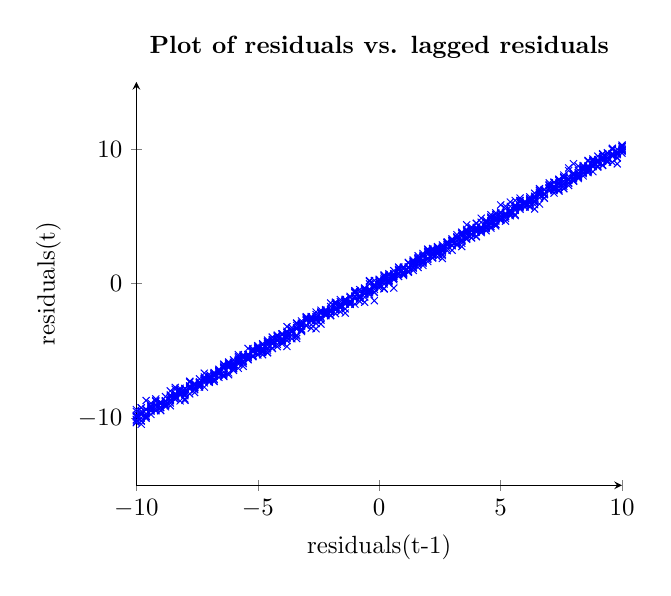
\begin{tikzpicture}[scale=0.9]
	\begin{axis}[
	xmin=-10, xmax=10, xlabel=residuals(t-1),
	ymin=-15, ymax=15, ylabel=residuals(t),
	samples=400,
	axis x line=bottom,
	axis y line=left,
	domain=-10:10,
	title=\textbf{Plot of residuals vs. lagged residuals}
	]
	\addplot[mark=x,blue, only marks] coordinates {
		(-10.00,-10.34)
		(-10.00,-10.28)
		(-10.00,-9.79)
		(-10.00,-10.14)
		(-10.00,-9.52)
		(-10.00,-9.84)
		(-10.00,-9.90)
		(-10.00,-9.37)
		(-10.00,-10.12)
		(-10.00,-9.89)
		(-9.80,-9.62)
		(-9.80,-9.99)
		(-9.80,-9.74)
		(-9.80,-10.23)
		(-9.80,-9.49)
		(-9.80,-9.23)
		(-9.80,-9.71)
		(-9.80,-10.46)
		(-9.80,-9.24)
		(-9.80,-10.18)
		(-9.60,-9.98)
		(-9.60,-9.86)
		(-9.60,-9.68)
		(-9.60,-10.02)
		(-9.60,-8.69)
		(-9.60,-9.88)
		(-9.60,-9.33)
		(-9.60,-9.39)
		(-9.60,-9.85)
		(-9.60,-9.88)
		(-9.40,-8.90)
		(-9.40,-9.18)
		(-9.40,-9.73)
		(-9.40,-9.48)
		(-9.40,-9.43)
		(-9.40,-9.21)
		(-9.40,-9.11)
		(-9.40,-9.10)
		(-9.40,-9.11)
		(-9.40,-9.31)
		(-9.20,-8.70)
		(-9.20,-9.45)
		(-9.20,-8.58)
		(-9.20,-9.00)
		(-9.20,-8.76)
		(-9.20,-9.27)
		(-9.20,-9.43)
		(-9.20,-9.04)
		(-9.20,-9.06)
		(-9.20,-9.05)
		(-9.00,-8.94)
		(-9.00,-8.80)
		(-9.00,-8.85)
		(-9.00,-9.23)
		(-9.00,-9.41)
		(-9.00,-8.86)
		(-9.00,-8.95)
		(-9.00,-8.85)
		(-9.00,-9.45)
		(-9.00,-9.19)
		(-8.80,-8.74)
		(-8.80,-8.40)
		(-8.80,-9.16)
		(-8.80,-8.76)
		(-8.80,-8.73)
		(-8.80,-8.71)
		(-8.80,-9.04)
		(-8.80,-9.05)
		(-8.80,-8.96)
		(-8.80,-8.78)
		(-8.60,-8.45)
		(-8.60,-7.98)
		(-8.60,-9.08)
		(-8.60,-8.30)
		(-8.60,-8.29)
		(-8.60,-8.63)
		(-8.60,-8.88)
		(-8.60,-8.70)
		(-8.60,-8.70)
		(-8.60,-8.43)
		(-8.40,-8.33)
		(-8.40,-8.19)
		(-8.40,-8.42)
		(-8.40,-8.22)
		(-8.40,-8.43)
		(-8.40,-7.86)
		(-8.40,-8.61)
		(-8.40,-8.18)
		(-8.40,-7.72)
		(-8.40,-8.57)
		(-8.20,-8.18)
		(-8.20,-7.97)
		(-8.20,-8.17)
		(-8.20,-7.91)
		(-8.20,-8.11)
		(-8.20,-7.79)
		(-8.20,-8.26)
		(-8.20,-8.72)
		(-8.20,-7.96)
		(-8.20,-8.31)
		(-8.00,-7.99)
		(-8.00,-7.81)
		(-8.00,-8.58)
		(-8.00,-8.11)
		(-8.00,-7.82)
		(-8.00,-8.68)
		(-8.00,-8.34)
		(-8.00,-8.24)
		(-8.00,-8.15)
		(-8.00,-7.80)
		(-7.80,-8.20)
		(-7.80,-7.84)
		(-7.80,-7.61)
		(-7.80,-7.66)
		(-7.80,-7.78)
		(-7.80,-7.63)
		(-7.80,-7.33)
		(-7.80,-7.76)
		(-7.80,-7.31)
		(-7.80,-7.26)
		(-7.60,-7.74)
		(-7.60,-7.72)
		(-7.60,-7.42)
		(-7.60,-7.83)
		(-7.60,-8.10)
		(-7.60,-7.52)
		(-7.60,-7.47)
		(-7.60,-7.54)
		(-7.60,-7.89)
		(-7.60,-7.72)
		(-7.40,-7.09)
		(-7.40,-7.35)
		(-7.40,-7.46)
		(-7.40,-7.57)
		(-7.40,-7.51)
		(-7.40,-7.39)
		(-7.40,-7.31)
		(-7.40,-7.61)
		(-7.40,-7.70)
		(-7.40,-7.39)
		(-7.20,-7.15)
		(-7.20,-7.19)
		(-7.20,-7.38)
		(-7.20,-7.70)
		(-7.20,-7.25)
		(-7.20,-6.94)
		(-7.20,-6.66)
		(-7.20,-7.04)
		(-7.20,-7.10)
		(-7.20,-7.06)
		(-7.00,-6.97)
		(-7.00,-7.24)
		(-7.00,-7.18)
		(-7.00,-7.34)
		(-7.00,-7.04)
		(-7.00,-6.94)
		(-7.00,-6.75)
		(-7.00,-7.12)
		(-7.00,-7.29)
		(-7.00,-6.90)
		(-6.80,-7.23)
		(-6.80,-7.11)
		(-6.80,-7.28)
		(-6.80,-6.78)
		(-6.80,-6.70)
		(-6.80,-7.10)
		(-6.80,-6.87)
		(-6.80,-6.61)
		(-6.80,-6.73)
		(-6.80,-6.88)
		(-6.60,-6.58)
		(-6.60,-6.65)
		(-6.60,-6.98)
		(-6.60,-6.45)
		(-6.60,-6.37)
		(-6.60,-6.52)
		(-6.60,-6.49)
		(-6.60,-6.48)
		(-6.60,-6.50)
		(-6.60,-6.74)
		(-6.40,-6.28)
		(-6.40,-6.25)
		(-6.40,-5.99)
		(-6.40,-6.91)
		(-6.40,-6.86)
		(-6.40,-6.20)
		(-6.40,-6.06)
		(-6.40,-6.31)
		(-6.40,-6.76)
		(-6.40,-6.57)
		(-6.20,-5.90)
		(-6.20,-5.83)
		(-6.20,-5.99)
		(-6.20,-6.64)
		(-6.20,-6.06)
		(-6.20,-6.78)
		(-6.20,-6.13)
		(-6.20,-6.24)
		(-6.20,-5.97)
		(-6.20,-6.24)
		(-6.00,-6.31)
		(-6.00,-6.09)
		(-6.00,-6.04)
		(-6.00,-6.45)
		(-6.00,-5.91)
		(-6.00,-6.26)
		(-6.00,-5.67)
		(-6.00,-5.85)
		(-6.00,-6.15)
		(-6.00,-6.33)
		(-5.80,-6.30)
		(-5.80,-5.53)
		(-5.80,-5.40)
		(-5.80,-5.72)
		(-5.80,-5.98)
		(-5.80,-5.66)
		(-5.80,-5.78)
		(-5.80,-5.72)
		(-5.80,-5.28)
		(-5.80,-5.86)
		(-5.60,-5.56)
		(-5.60,-5.95)
		(-5.60,-5.82)
		(-5.60,-5.29)
		(-5.60,-5.76)
		(-5.60,-6.15)
		(-5.60,-5.43)
		(-5.60,-5.43)
		(-5.60,-5.44)
		(-5.60,-5.35)
		(-5.40,-5.60)
		(-5.40,-5.29)
		(-5.40,-5.48)
		(-5.40,-5.27)
		(-5.40,-5.66)
		(-5.40,-5.32)
		(-5.40,-5.46)
		(-5.40,-4.82)
		(-5.40,-5.44)
		(-5.40,-5.27)
		(-5.20,-5.06)
		(-5.20,-5.35)
		(-5.20,-4.84)
		(-5.20,-5.08)
		(-5.20,-4.89)
		(-5.20,-5.40)
		(-5.20,-5.44)
		(-5.20,-5.04)
		(-5.20,-4.99)
		(-5.20,-5.02)
		(-5.00,-4.71)
		(-5.00,-4.98)
		(-5.00,-5.03)
		(-5.00,-5.31)
		(-5.00,-4.97)
		(-5.00,-4.83)
		(-5.00,-4.62)
		(-5.00,-5.22)
		(-5.00,-4.86)
		(-5.00,-4.78)
		(-4.80,-4.47)
		(-4.80,-4.84)
		(-4.80,-5.12)
		(-4.80,-4.93)
		(-4.80,-5.04)
		(-4.80,-4.81)
		(-4.80,-5.29)
		(-4.80,-5.00)
		(-4.80,-4.98)
		(-4.80,-4.57)
		(-4.60,-4.31)
		(-4.60,-4.44)
		(-4.60,-4.80)
		(-4.60,-4.77)
		(-4.60,-5.11)
		(-4.60,-4.20)
		(-4.60,-5.15)
		(-4.60,-4.35)
		(-4.60,-4.94)
		(-4.60,-4.58)
		(-4.40,-4.47)
		(-4.40,-4.16)
		(-4.40,-3.98)
		(-4.40,-4.48)
		(-4.40,-4.00)
		(-4.40,-4.83)
		(-4.40,-4.80)
		(-4.40,-4.20)
		(-4.40,-4.24)
		(-4.40,-4.35)
		(-4.20,-4.69)
		(-4.20,-3.97)
		(-4.20,-3.83)
		(-4.20,-4.15)
		(-4.20,-4.25)
		(-4.20,-4.51)
		(-4.20,-4.26)
		(-4.20,-3.89)
		(-4.20,-4.17)
		(-4.20,-4.20)
		(-4.00,-3.83)
		(-4.00,-4.23)
		(-4.00,-4.12)
		(-4.00,-4.37)
		(-4.00,-4.48)
		(-4.00,-4.11)
		(-4.00,-3.74)
		(-4.00,-4.12)
		(-4.00,-3.73)
		(-4.00,-4.25)
		(-3.80,-3.83)
		(-3.80,-4.02)
		(-3.80,-3.66)
		(-3.80,-3.63)
		(-3.80,-3.96)
		(-3.80,-4.06)
		(-3.80,-4.67)
		(-3.80,-4.24)
		(-3.80,-3.54)
		(-3.80,-3.20)
		(-3.60,-3.48)
		(-3.60,-3.59)
		(-3.60,-3.44)
		(-3.60,-4.10)
		(-3.60,-3.28)
		(-3.60,-3.55)
		(-3.60,-3.85)
		(-3.60,-3.60)
		(-3.60,-3.58)
		(-3.60,-3.57)
		(-3.40,-3.11)
		(-3.40,-3.36)
		(-3.40,-3.36)
		(-3.40,-2.97)
		(-3.40,-4.08)
		(-3.40,-3.28)
		(-3.40,-3.83)
		(-3.40,-3.33)
		(-3.40,-2.93)
		(-3.40,-3.91)
		(-3.20,-3.17)
		(-3.20,-3.43)
		(-3.20,-2.95)
		(-3.20,-3.11)
		(-3.20,-3.56)
		(-3.20,-3.02)
		(-3.20,-2.96)
		(-3.20,-3.48)
		(-3.20,-3.38)
		(-3.20,-2.78)
		(-3.00,-3.10)
		(-3.00,-2.73)
		(-3.00,-2.55)
		(-3.00,-2.72)
		(-3.00,-2.58)
		(-3.00,-3.13)
		(-3.00,-2.73)
		(-3.00,-2.54)
		(-3.00,-2.65)
		(-3.00,-2.46)
		(-2.80,-3.31)
		(-2.80,-2.56)
		(-2.80,-2.74)
		(-2.80,-2.73)
		(-2.80,-2.45)
		(-2.80,-2.80)
		(-2.80,-2.61)
		(-2.80,-3.06)
		(-2.80,-2.75)
		(-2.80,-2.63)
		(-2.60,-2.59)
		(-2.60,-2.74)
		(-2.60,-2.30)
		(-2.60,-2.12)
		(-2.60,-2.46)
		(-2.60,-2.96)
		(-2.60,-2.59)
		(-2.60,-2.63)
		(-2.60,-3.36)
		(-2.60,-2.69)
		(-2.40,-2.21)
		(-2.40,-2.19)
		(-2.40,-3.01)
		(-2.40,-2.48)
		(-2.40,-2.15)
		(-2.40,-2.59)
		(-2.40,-2.19)
		(-2.40,-2.71)
		(-2.40,-2.12)
		(-2.40,-1.98)
		(-2.20,-1.96)
		(-2.20,-2.25)
		(-2.20,-2.21)
		(-2.20,-2.39)
		(-2.20,-2.33)
		(-2.20,-2.01)
		(-2.20,-2.18)
		(-2.20,-2.15)
		(-2.20,-1.94)
		(-2.20,-2.03)
		(-2.00,-1.93)
		(-2.00,-1.70)
		(-2.00,-1.98)
		(-2.00,-2.39)
		(-2.00,-2.03)
		(-2.00,-1.44)
		(-2.00,-2.07)
		(-2.00,-2.35)
		(-2.00,-1.94)
		(-2.00,-2.13)
		(-1.80,-1.55)
		(-1.80,-1.44)
		(-1.80,-1.83)
		(-1.80,-1.50)
		(-1.80,-1.90)
		(-1.80,-1.95)
		(-1.80,-2.23)
		(-1.80,-1.94)
		(-1.80,-1.38)
		(-1.80,-1.72)
		(-1.60,-1.80)
		(-1.60,-1.78)
		(-1.60,-1.74)
		(-1.60,-1.34)
		(-1.60,-1.60)
		(-1.60,-1.54)
		(-1.60,-1.55)
		(-1.60,-1.63)
		(-1.60,-2.09)
		(-1.60,-1.19)
		(-1.40,-1.88)
		(-1.40,-2.19)
		(-1.40,-1.53)
		(-1.40,-1.18)
		(-1.40,-1.41)
		(-1.40,-1.48)
		(-1.40,-1.45)
		(-1.40,-1.28)
		(-1.40,-1.28)
		(-1.40,-1.17)
		(-1.20,-1.43)
		(-1.20,-1.48)
		(-1.20,-0.95)
		(-1.20,-1.29)
		(-1.20,-1.41)
		(-1.20,-1.54)
		(-1.20,-1.51)
		(-1.20,-1.31)
		(-1.20,-1.03)
		(-1.20,-1.53)
		(-1.00,-0.54)
		(-1.00,-0.55)
		(-1.00,-0.63)
		(-1.00,-0.97)
		(-1.00,-1.13)
		(-1.00,-0.68)
		(-1.00,-0.99)
		(-1.00,-0.92)
		(-1.00,-0.68)
		(-1.00,-1.53)
		(-0.80,-0.45)
		(-0.80,-0.95)
		(-0.80,-1.32)
		(-0.80,-0.88)
		(-0.80,-1.08)
		(-0.80,-1.06)
		(-0.80,-1.09)
		(-0.80,-0.62)
		(-0.80,-1.02)
		(-0.80,-0.97)
		(-0.60,-0.56)
		(-0.60,-1.01)
		(-0.60,-0.33)
		(-0.60,-1.39)
		(-0.60,-0.72)
		(-0.60,-0.78)
		(-0.60,-0.39)
		(-0.60,-0.48)
		(-0.60,-0.42)
		(-0.60,-0.75)
		(-0.40,0.16)
		(-0.40,-0.54)
		(-0.40,-0.40)
		(-0.40,-0.61)
		(-0.40,-0.02)
		(-0.40,-0.69)
		(-0.40,-0.83)
		(-0.40,-0.49)
		(-0.40,0.22)
		(-0.40,-0.48)
		(-0.20,-0.43)
		(-0.20,-0.20)
		(-0.20,-0.13)
		(-0.20,-0.29)
		(-0.20,-0.06)
		(-0.20,-0.66)
		(-0.20,-0.63)
		(-0.20,-1.27)
		(-0.20,-0.18)
		(-0.20,0.23)
		(0.00,0.07)
		(0.00,0.04)
		(0.00,0.25)
		(0.00,-0.10)
		(0.00,-0.18)
		(0.00,0.08)
		(0.00,0.22)
		(0.00,0.32)
		(0.00,-0.33)
		(0.00,-0.07)
		(0.20,-0.36)
		(0.20,0.14)
		(0.20,-0.03)
		(0.20,0.33)
		(0.20,0.34)
		(0.20,0.49)
		(0.20,0.60)
		(0.20,0.64)
		(0.20,-0.40)
		(0.20,0.21)
		(0.40,0.02)
		(0.40,0.62)
		(0.40,0.22)
		(0.40,0.21)
		(0.40,0.23)
		(0.40,0.13)
		(0.40,0.29)
		(0.40,0.73)
		(0.40,0.63)
		(0.40,0.43)
		(0.60,0.52)
		(0.60,-0.33)
		(0.60,0.41)
		(0.60,0.71)
		(0.60,0.72)
		(0.60,0.69)
		(0.60,0.28)
		(0.60,0.57)
		(0.60,0.38)
		(0.60,0.96)
		(0.80,1.22)
		(0.80,1.07)
		(0.80,0.76)
		(0.80,0.99)
		(0.80,0.53)
		(0.80,1.22)
		(0.80,1.03)
		(0.80,0.68)
		(0.80,0.99)
		(0.80,0.78)
		(1.00,1.18)
		(1.00,0.79)
		(1.00,1.07)
		(1.00,0.80)
		(1.00,0.60)
		(1.00,0.79)
		(1.00,0.85)
		(1.00,1.23)
		(1.00,0.68)
		(1.00,1.19)
		(1.20,0.92)
		(1.20,1.52)
		(1.20,1.23)
		(1.20,1.16)
		(1.20,0.84)
		(1.20,0.86)
		(1.20,1.13)
		(1.20,1.58)
		(1.20,1.22)
		(1.20,0.90)
		(1.40,1.67)
		(1.40,1.37)
		(1.40,1.66)
		(1.40,1.23)
		(1.40,1.46)
		(1.40,0.98)
		(1.40,1.15)
		(1.40,1.61)
		(1.40,1.56)
		(1.40,1.76)
		(1.60,1.75)
		(1.60,1.65)
		(1.60,1.82)
		(1.60,1.84)
		(1.60,1.94)
		(1.60,2.07)
		(1.60,1.83)
		(1.60,1.55)
		(1.60,1.20)
		(1.60,1.40)
		(1.80,1.55)
		(1.80,1.63)
		(1.80,2.24)
		(1.80,1.52)
		(1.80,2.00)
		(1.80,1.35)
		(1.80,1.71)
		(1.80,1.78)
		(1.80,1.63)
		(1.80,2.10)
		(2.00,1.90)
		(2.00,2.37)
		(2.00,1.80)
		(2.00,1.64)
		(2.00,2.18)
		(2.00,2.57)
		(2.00,2.40)
		(2.00,2.32)
		(2.00,2.19)
		(2.00,2.51)
		(2.20,2.61)
		(2.20,2.11)
		(2.20,2.24)
		(2.20,1.94)
		(2.20,2.15)
		(2.20,2.44)
		(2.20,2.32)
		(2.20,1.90)
		(2.20,2.58)
		(2.20,2.50)
		(2.40,2.75)
		(2.40,2.49)
		(2.40,2.69)
		(2.40,2.55)
		(2.40,2.57)
		(2.40,2.38)
		(2.40,2.29)
		(2.40,1.99)
		(2.40,2.36)
		(2.40,2.21)
		(2.60,2.38)
		(2.60,2.49)
		(2.60,2.72)
		(2.60,2.19)
		(2.60,2.65)
		(2.60,2.50)
		(2.60,2.08)
		(2.60,1.87)
		(2.60,2.87)
		(2.60,2.47)
		(2.80,3.00)
		(2.80,2.88)
		(2.80,2.63)
		(2.80,3.05)
		(2.80,3.05)
		(2.80,2.85)
		(2.80,3.10)
		(2.80,2.91)
		(2.80,3.02)
		(2.80,2.45)
		(3.00,3.32)
		(3.00,2.48)
		(3.00,2.85)
		(3.00,3.18)
		(3.00,2.86)
		(3.00,3.14)
		(3.00,3.17)
		(3.00,2.81)
		(3.00,3.23)
		(3.00,3.08)
		(3.20,3.21)
		(3.20,3.48)
		(3.20,3.15)
		(3.20,2.90)
		(3.20,3.38)
		(3.20,3.42)
		(3.20,2.96)
		(3.20,3.64)
		(3.20,2.86)
		(3.20,2.94)
		(3.40,3.56)
		(3.40,2.75)
		(3.40,3.00)
		(3.40,3.28)
		(3.40,3.75)
		(3.40,3.82)
		(3.40,3.15)
		(3.40,3.20)
		(3.40,3.51)
		(3.40,3.69)
		(3.60,4.37)
		(3.60,3.70)
		(3.60,3.84)
		(3.60,3.47)
		(3.60,3.30)
		(3.60,3.64)
		(3.60,3.68)
		(3.60,3.36)
		(3.60,3.95)
		(3.60,4.03)
		(3.80,3.92)
		(3.80,4.21)
		(3.80,3.64)
		(3.80,3.40)
		(3.80,3.41)
		(3.80,3.92)
		(3.80,3.70)
		(3.80,3.93)
		(3.80,4.12)
		(3.80,3.96)
		(4.00,4.18)
		(4.00,3.49)
		(4.00,3.84)
		(4.00,3.93)
		(4.00,4.46)
		(4.00,4.06)
		(4.00,3.53)
		(4.00,4.49)
		(4.00,4.15)
		(4.00,4.00)
		(4.20,4.06)
		(4.20,4.56)
		(4.20,3.95)
		(4.20,4.86)
		(4.20,4.15)
		(4.20,3.91)
		(4.20,3.79)
		(4.20,4.11)
		(4.20,4.21)
		(4.20,4.09)
		(4.40,4.19)
		(4.40,4.57)
		(4.40,4.17)
		(4.40,4.48)
		(4.40,4.32)
		(4.40,4.59)
		(4.40,3.93)
		(4.40,4.69)
		(4.40,4.09)
		(4.40,4.14)
		(4.60,4.90)
		(4.60,5.12)
		(4.60,4.47)
		(4.60,4.66)
		(4.60,4.24)
		(4.60,4.12)
		(4.60,4.95)
		(4.60,4.82)
		(4.60,4.59)
		(4.60,4.44)
		(4.80,4.43)
		(4.80,4.63)
		(4.80,5.25)
		(4.80,4.73)
		(4.80,4.97)
		(4.80,4.83)
		(4.80,4.40)
		(4.80,4.29)
		(4.80,5.12)
		(4.80,4.87)
		(5.00,5.85)
		(5.00,4.96)
		(5.00,5.20)
		(5.00,5.04)
		(5.00,4.81)
		(5.00,4.76)
		(5.00,4.70)
		(5.00,5.30)
		(5.00,4.83)
		(5.00,4.71)
		(5.20,5.15)
		(5.20,5.00)
		(5.20,5.17)
		(5.20,4.64)
		(5.20,4.84)
		(5.20,5.22)
		(5.20,4.97)
		(5.20,5.01)
		(5.20,5.75)
		(5.20,5.58)
		(5.40,5.33)
		(5.40,5.04)
		(5.40,5.12)
		(5.40,6.06)
		(5.40,5.36)
		(5.40,5.48)
		(5.40,5.41)
		(5.40,5.74)
		(5.40,5.17)
		(5.40,5.18)
		(5.60,5.06)
		(5.60,5.14)
		(5.60,5.68)
		(5.60,5.57)
		(5.60,5.83)
		(5.60,5.45)
		(5.60,5.74)
		(5.60,5.82)
		(5.60,6.18)
		(5.60,5.57)
		(5.80,5.74)
		(5.80,5.83)
		(5.80,5.82)
		(5.80,5.75)
		(5.80,6.36)
		(5.80,6.17)
		(5.80,5.64)
		(5.80,6.05)
		(5.80,6.17)
		(5.80,5.52)
		(6.00,5.68)
		(6.00,5.90)
		(6.00,6.07)
		(6.00,6.04)
		(6.00,5.97)
		(6.00,6.06)
		(6.00,5.71)
		(6.00,5.74)
		(6.00,6.10)
		(6.00,5.94)
		(6.20,6.08)
		(6.20,5.69)
		(6.20,6.26)
		(6.20,6.31)
		(6.20,5.78)
		(6.20,6.14)
		(6.20,6.19)
		(6.20,6.44)
		(6.20,5.98)
		(6.20,6.01)
		(6.40,6.16)
		(6.40,5.87)
		(6.40,6.42)
		(6.40,6.49)
		(6.40,6.16)
		(6.40,6.11)
		(6.40,6.05)
		(6.40,6.34)
		(6.40,6.72)
		(6.40,5.55)
		(6.60,5.92)
		(6.60,6.91)
		(6.60,6.38)
		(6.60,6.58)
		(6.60,6.95)
		(6.60,7.06)
		(6.60,6.61)
		(6.60,6.80)
		(6.60,6.66)
		(6.60,6.74)
		(6.80,6.69)
		(6.80,6.35)
		(6.80,6.97)
		(6.80,6.99)
		(6.80,6.68)
		(6.80,6.63)
		(6.80,6.36)
		(6.80,6.64)
		(6.80,6.62)
		(6.80,6.69)
		(7.00,7.49)
		(7.00,7.11)
		(7.00,6.88)
		(7.00,7.09)
		(7.00,7.09)
		(7.00,7.35)
		(7.00,7.26)
		(7.00,7.30)
		(7.00,7.05)
		(7.00,7.11)
		(7.20,7.52)
		(7.20,7.23)
		(7.20,6.73)
		(7.20,7.25)
		(7.20,6.92)
		(7.20,7.18)
		(7.20,7.06)
		(7.20,6.99)
		(7.20,7.54)
		(7.20,7.08)
		(7.40,7.40)
		(7.40,7.42)
		(7.40,6.97)
		(7.40,7.75)
		(7.40,7.36)
		(7.40,7.64)
		(7.40,7.48)
		(7.40,7.74)
		(7.40,7.18)
		(7.40,6.88)
		(7.60,7.45)
		(7.60,7.41)
		(7.60,7.24)
		(7.60,7.94)
		(7.60,7.88)
		(7.60,7.85)
		(7.60,7.05)
		(7.60,7.08)
		(7.60,8.07)
		(7.60,7.62)
		(7.80,7.96)
		(7.80,7.70)
		(7.80,7.29)
		(7.80,7.78)
		(7.80,7.72)
		(7.80,8.60)
		(7.80,7.45)
		(7.80,7.68)
		(7.80,7.51)
		(7.80,8.40)
		(8.00,8.21)
		(8.00,7.63)
		(8.00,8.10)
		(8.00,7.61)
		(8.00,7.90)
		(8.00,8.91)
		(8.00,8.10)
		(8.00,7.68)
		(8.00,8.07)
		(8.00,7.80)
		(8.20,7.89)
		(8.20,7.92)
		(8.20,8.23)
		(8.20,8.43)
		(8.20,8.18)
		(8.20,7.81)
		(8.20,7.97)
		(8.20,8.73)
		(8.20,8.00)
		(8.20,8.06)
		(8.40,8.78)
		(8.40,8.00)
		(8.40,8.61)
		(8.40,8.27)
		(8.40,8.18)
		(8.40,8.69)
		(8.40,8.44)
		(8.40,8.50)
		(8.40,8.50)
		(8.40,8.46)
		(8.60,8.34)
		(8.60,8.25)
		(8.60,8.76)
		(8.60,8.44)
		(8.60,9.10)
		(8.60,8.51)
		(8.60,8.71)
		(8.60,9.16)
		(8.60,8.59)
		(8.60,8.71)
		(8.80,8.74)
		(8.80,9.26)
		(8.80,8.88)
		(8.80,9.15)
		(8.80,8.69)
		(8.80,8.32)
		(8.80,8.79)
		(8.80,9.16)
		(8.80,9.03)
		(8.80,8.73)
		(9.00,9.00)
		(9.00,8.72)
		(9.00,9.21)
		(9.00,8.76)
		(9.00,9.10)
		(9.00,8.66)
		(9.00,9.03)
		(9.00,9.47)
		(9.00,9.04)
		(9.00,9.12)
		(9.20,9.12)
		(9.20,8.82)
		(9.20,9.59)
		(9.20,9.65)
		(9.20,9.30)
		(9.20,9.32)
		(9.20,9.30)
		(9.20,8.78)
		(9.20,9.24)
		(9.20,9.42)
		(9.40,9.03)
		(9.40,9.73)
		(9.40,9.14)
		(9.40,9.37)
		(9.40,9.14)
		(9.40,9.30)
		(9.40,9.69)
		(9.40,9.13)
		(9.40,9.53)
		(9.40,9.34)
		(9.60,9.66)
		(9.60,9.47)
		(9.60,9.96)
		(9.60,10.06)
		(9.60,9.62)
		(9.60,9.02)
		(9.60,9.62)
		(9.60,10.01)
		(9.60,9.65)
		(9.60,9.49)
		(9.80,9.77)
		(9.80,8.90)
		(9.80,9.73)
		(9.80,9.66)
		(9.80,9.68)
		(9.80,9.78)
		(9.80,9.38)
		(9.80,9.32)
		(9.80,9.98)
		(9.80,9.59)
		(10.00,9.85)
		(10.00,10.21)
		(10.00,9.90)
		(10.00,10.21)
		(10.00,10.07)
		(10.00,9.91)
		(10.00,9.97)
		(10.00,9.70)
		(10.00,10.19)
		(10.00,10.30)
	};
	\end{axis}
	\end{tikzpicture}
\end{center}

\subsection{Hypothesis testing on simple linear model parameters}

How to test if the $x_i$s contribute information for the prediction of $Y$ in $Y_i=\beta_0+\beta_1x_i+\epsilon_i$? One way of doing this is to test the hypothesis that $Y$ does not change as the explanatory $x$ changes. In other words, we test the hypothesis \\
$H_0$: $\beta_1=0$ \\
$H_A$: $\beta_1\neq 0$ \\
Fortunately, 'math boffins' have found that $\hat{\beta_1}$ follows a normal distribution with mean $\beta_1$ and standard error 
\begin{align}
	\sigma_{\hat{\beta_1}} = \frac{\sigma}{\sqrt{SS_{xx}}}\approx \frac{s}{\sqrt{SS_{xx}}}\notag
\end{align}
where $SS_{xx}=\sum(x_i-\bar{x})^2$ and $s^2=\frac{\sum (Y_i-\hat{Y_i})^2}{n-2}$. Since $\sigma$ is usually unknown, we need to use a \person{Student}'s t-test on
\begin{align}
	t = \frac{\hat{\beta_1}-\text{hypothesised value}}{\frac{s}{\sqrt{SS_{xx}}}} \notag
\end{align}
with degrees of freedom based on the number of data points and model parameters. In practice, software will does this for us!

As an alternative for interference on parameter estimates, we can also compute confidence intervals. The $(1-\alpha)100\%$ confidence interval for the gradient $\beta_1$ is
\begin{align}
	\hat{\beta_1}\pm t_{\nicefrac{\alpha}{2}}s_{\hat{\beta_1}}\notag 
\end{align}
where $s_{\hat{\beta_1}} = \frac{s}{\sqrt{SS_{xx}}}$ and $t_{\nicefrac{\alpha}{2}}$ is based on $n-2$ degrees of freedom. $t_{\nicefrac{\alpha}{2}}$ is obtained from the \person{Stundent}'s t-distribution in the usual way. Some statistical software provides these values by default, but often (e.g. in MATLAB), only the standard errors for parameter estimates are provided.

\subsection{Estimation and prediction for simple linear models}

\begin{definition}[estimation]
	\begriff[simple linear models!]{Estimation}: estimate mean value of $Y$ over many data points
\end{definition}

\begin{definition}[prediction]
	\begriff[simple linear models!]{Prediction}: predict $Y$ for a particular value of $x$. This leads to higher error bounds (add error in mean to variation around mean).
\end{definition}

\begin{center}
	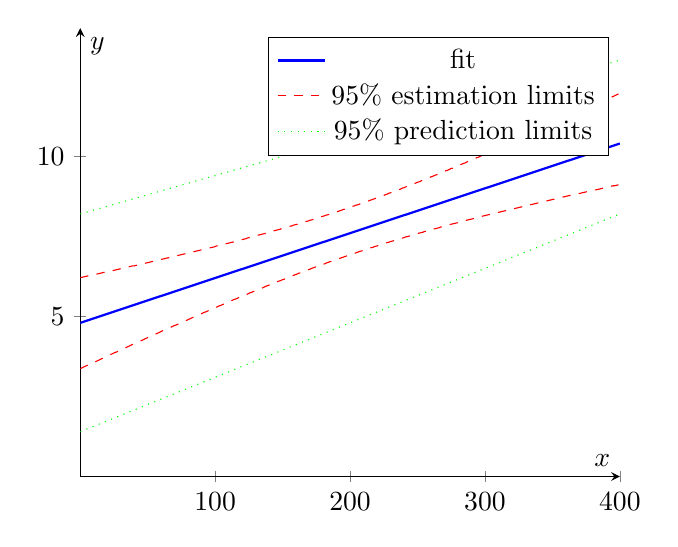
\begin{tikzpicture}
	\begin{axis}[
	xmin=0, xmax=400, xlabel=$x$,
	ymin=0, ymax=14, ylabel=$y$,
	axis x line=middle,
	axis y line=middle,
	domain=0:400,
	samples=400
	]
	\addplot[thick, blue] {0.014*x+4.8};
	\addlegendentry {fit};
	\addplot[red,dashed] coordinates {
		(0.00,3.37)
		(1.00,3.39)
		(2.00,3.41)
		(3.00,3.43)
		(4.00,3.45)
		(5.00,3.47)
		(6.00,3.49)
		(7.00,3.51)
		(8.00,3.53)
		(9.00,3.55)
		(10.00,3.56)
		(11.00,3.58)
		(12.00,3.60)
		(13.00,3.62)
		(14.00,3.64)
		(15.00,3.66)
		(16.00,3.68)
		(17.00,3.70)
		(18.00,3.72)
		(19.00,3.74)
		(20.00,3.76)
		(21.00,3.78)
		(22.00,3.80)
		(23.00,3.82)
		(24.00,3.84)
		(25.00,3.86)
		(26.00,3.88)
		(27.00,3.89)
		(28.00,3.91)
		(29.00,3.93)
		(30.00,3.95)
		(31.00,3.97)
		(32.00,3.99)
		(33.00,4.01)
		(34.00,4.03)
		(35.00,4.05)
		(36.00,4.07)
		(37.00,4.09)
		(38.00,4.11)
		(39.00,4.13)
		(40.00,4.15)
		(41.00,4.16)
		(42.00,4.18)
		(43.00,4.20)
		(44.00,4.22)
		(45.00,4.24)
		(46.00,4.26)
		(47.00,4.28)
		(48.00,4.30)
		(49.00,4.32)
		(50.00,4.34)
		(51.00,4.36)
		(52.00,4.38)
		(53.00,4.39)
		(54.00,4.41)
		(55.00,4.43)
		(56.00,4.45)
		(57.00,4.47)
		(58.00,4.49)
		(59.00,4.51)
		(60.00,4.53)
		(61.00,4.55)
		(62.00,4.57)
		(63.00,4.58)
		(64.00,4.60)
		(65.00,4.62)
		(66.00,4.64)
		(67.00,4.66)
		(68.00,4.68)
		(69.00,4.70)
		(70.00,4.72)
		(71.00,4.73)
		(72.00,4.75)
		(73.00,4.77)
		(74.00,4.79)
		(75.00,4.81)
		(76.00,4.83)
		(77.00,4.85)
		(78.00,4.87)
		(79.00,4.88)
		(80.00,4.90)
		(81.00,4.92)
		(82.00,4.94)
		(83.00,4.96)
		(84.00,4.98)
		(85.00,5.00)
		(86.00,5.01)
		(87.00,5.03)
		(88.00,5.05)
		(89.00,5.07)
		(90.00,5.09)
		(91.00,5.11)
		(92.00,5.13)
		(93.00,5.14)
		(94.00,5.16)
		(95.00,5.18)
		(96.00,5.20)
		(97.00,5.22)
		(98.00,5.24)
		(99.00,5.25)
		(100.00,5.27)
		(101.00,5.29)
		(102.00,5.31)
		(103.00,5.33)
		(104.00,5.34)
		(105.00,5.36)
		(106.00,5.38)
		(107.00,5.40)
		(108.00,5.42)
		(109.00,5.44)
		(110.00,5.45)
		(111.00,5.47)
		(112.00,5.49)
		(113.00,5.51)
		(114.00,5.53)
		(115.00,5.54)
		(116.00,5.56)
		(117.00,5.58)
		(118.00,5.60)
		(119.00,5.61)
		(120.00,5.63)
		(121.00,5.65)
		(122.00,5.67)
		(123.00,5.68)
		(124.00,5.70)
		(125.00,5.72)
		(126.00,5.74)
		(127.00,5.75)
		(128.00,5.77)
		(129.00,5.79)
		(130.00,5.81)
		(131.00,5.82)
		(132.00,5.84)
		(133.00,5.86)
		(134.00,5.88)
		(135.00,5.89)
		(136.00,5.91)
		(137.00,5.93)
		(138.00,5.95)
		(139.00,5.96)
		(140.00,5.98)
		(141.00,6.00)
		(142.00,6.01)
		(143.00,6.03)
		(144.00,6.05)
		(145.00,6.06)
		(146.00,6.08)
		(147.00,6.10)
		(148.00,6.11)
		(149.00,6.13)
		(150.00,6.15)
		(151.00,6.16)
		(152.00,6.18)
		(153.00,6.20)
		(154.00,6.21)
		(155.00,6.23)
		(156.00,6.25)
		(157.00,6.26)
		(158.00,6.28)
		(159.00,6.30)
		(160.00,6.31)
		(161.00,6.33)
		(162.00,6.35)
		(163.00,6.36)
		(164.00,6.38)
		(165.00,6.39)
		(166.00,6.41)
		(167.00,6.43)
		(168.00,6.44)
		(169.00,6.46)
		(170.00,6.47)
		(171.00,6.49)
		(172.00,6.51)
		(173.00,6.52)
		(174.00,6.54)
		(175.00,6.55)
		(176.00,6.57)
		(177.00,6.58)
		(178.00,6.60)
		(179.00,6.61)
		(180.00,6.63)
		(181.00,6.64)
		(182.00,6.66)
		(183.00,6.68)
		(184.00,6.69)
		(185.00,6.71)
		(186.00,6.72)
		(187.00,6.74)
		(188.00,6.75)
		(189.00,6.77)
		(190.00,6.78)
		(191.00,6.80)
		(192.00,6.81)
		(193.00,6.82)
		(194.00,6.84)
		(195.00,6.85)
		(196.00,6.87)
		(197.00,6.88)
		(198.00,6.90)
		(199.00,6.91)
		(200.00,6.93)
		(201.00,6.94)
		(202.00,6.96)
		(203.00,6.97)
		(204.00,6.98)
		(205.00,7.00)
		(206.00,7.01)
		(207.00,7.03)
		(208.00,7.04)
		(209.00,7.05)
		(210.00,7.07)
		(211.00,7.08)
		(212.00,7.10)
		(213.00,7.11)
		(214.00,7.12)
		(215.00,7.14)
		(216.00,7.15)
		(217.00,7.16)
		(218.00,7.18)
		(219.00,7.19)
		(220.00,7.20)
		(221.00,7.22)
		(222.00,7.23)
		(223.00,7.24)
		(224.00,7.26)
		(225.00,7.27)
		(226.00,7.28)
		(227.00,7.30)
		(228.00,7.31)
		(229.00,7.32)
		(230.00,7.34)
		(231.00,7.35)
		(232.00,7.36)
		(233.00,7.37)
		(234.00,7.39)
		(235.00,7.40)
		(236.00,7.41)
		(237.00,7.43)
		(238.00,7.44)
		(239.00,7.45)
		(240.00,7.46)
		(241.00,7.48)
		(242.00,7.49)
		(243.00,7.50)
		(244.00,7.51)
		(245.00,7.52)
		(246.00,7.54)
		(247.00,7.55)
		(248.00,7.56)
		(249.00,7.57)
		(250.00,7.59)
		(251.00,7.60)
		(252.00,7.61)
		(253.00,7.62)
		(254.00,7.63)
		(255.00,7.65)
		(256.00,7.66)
		(257.00,7.67)
		(258.00,7.68)
		(259.00,7.69)
		(260.00,7.70)
		(261.00,7.72)
		(262.00,7.73)
		(263.00,7.74)
		(264.00,7.75)
		(265.00,7.76)
		(266.00,7.77)
		(267.00,7.79)
		(268.00,7.80)
		(269.00,7.81)
		(270.00,7.82)
		(271.00,7.83)
		(272.00,7.84)
		(273.00,7.85)
		(274.00,7.87)
		(275.00,7.88)
		(276.00,7.89)
		(277.00,7.90)
		(278.00,7.91)
		(279.00,7.92)
		(280.00,7.93)
		(281.00,7.94)
		(282.00,7.95)
		(283.00,7.96)
		(284.00,7.98)
		(285.00,7.99)
		(286.00,8.00)
		(287.00,8.01)
		(288.00,8.02)
		(289.00,8.03)
		(290.00,8.04)
		(291.00,8.05)
		(292.00,8.06)
		(293.00,8.07)
		(294.00,8.08)
		(295.00,8.09)
		(296.00,8.11)
		(297.00,8.12)
		(298.00,8.13)
		(299.00,8.14)
		(300.00,8.15)
		(301.00,8.16)
		(302.00,8.17)
		(303.00,8.18)
		(304.00,8.19)
		(305.00,8.20)
		(306.00,8.21)
		(307.00,8.22)
		(308.00,8.23)
		(309.00,8.24)
		(310.00,8.25)
		(311.00,8.26)
		(312.00,8.27)
		(313.00,8.28)
		(314.00,8.29)
		(315.00,8.30)
		(316.00,8.31)
		(317.00,8.32)
		(318.00,8.33)
		(319.00,8.34)
		(320.00,8.35)
		(321.00,8.36)
		(322.00,8.37)
		(323.00,8.38)
		(324.00,8.39)
		(325.00,8.40)
		(326.00,8.41)
		(327.00,8.42)
		(328.00,8.43)
		(329.00,8.44)
		(330.00,8.45)
		(331.00,8.46)
		(332.00,8.47)
		(333.00,8.48)
		(334.00,8.49)
		(335.00,8.50)
		(336.00,8.51)
		(337.00,8.52)
		(338.00,8.53)
		(339.00,8.54)
		(340.00,8.55)
		(341.00,8.56)
		(342.00,8.57)
		(343.00,8.58)
		(344.00,8.59)
		(345.00,8.60)
		(346.00,8.61)
		(347.00,8.62)
		(348.00,8.63)
		(349.00,8.64)
		(350.00,8.65)
		(351.00,8.66)
		(352.00,8.67)
		(353.00,8.68)
		(354.00,8.69)
		(355.00,8.70)
		(356.00,8.71)
		(357.00,8.72)
		(358.00,8.73)
		(359.00,8.74)
		(360.00,8.75)
		(361.00,8.76)
		(362.00,8.77)
		(363.00,8.78)
		(364.00,8.78)
		(365.00,8.79)
		(366.00,8.80)
		(367.00,8.81)
		(368.00,8.82)
		(369.00,8.83)
		(370.00,8.84)
		(371.00,8.85)
		(372.00,8.86)
		(373.00,8.87)
		(374.00,8.88)
		(375.00,8.89)
		(376.00,8.90)
		(377.00,8.91)
		(378.00,8.92)
		(379.00,8.93)
		(380.00,8.94)
		(381.00,8.95)
		(382.00,8.95)
		(383.00,8.96)
		(384.00,8.97)
		(385.00,8.98)
		(386.00,8.99)
		(387.00,9.00)
		(388.00,9.01)
		(389.00,9.02)
		(390.00,9.03)
		(391.00,9.04)
		(392.00,9.05)
		(393.00,9.06)
		(394.00,9.07)
		(395.00,9.08)
		(396.00,9.08)
		(397.00,9.09)
		(398.00,9.10)
		(399.00,9.11)
	};
	\addlegendentry {95\% estimation limits};
	\addplot[green,dotted] {x*-5.7*10^-6*x+0.017*x+1.4};
	\addlegendentry {95\% prediction limits};
	\addplot[red,dashed] coordinates {
		(0.00,6.21)
		(1.00,6.22)
		(2.00,6.23)
		(3.00,6.24)
		(4.00,6.25)
		(5.00,6.26)
		(6.00,6.27)
		(7.00,6.27)
		(8.00,6.28)
		(9.00,6.29)
		(10.00,6.30)
		(11.00,6.31)
		(12.00,6.32)
		(13.00,6.33)
		(14.00,6.34)
		(15.00,6.35)
		(16.00,6.36)
		(17.00,6.37)
		(18.00,6.38)
		(19.00,6.39)
		(20.00,6.40)
		(21.00,6.40)
		(22.00,6.41)
		(23.00,6.42)
		(24.00,6.43)
		(25.00,6.44)
		(26.00,6.45)
		(27.00,6.46)
		(28.00,6.47)
		(29.00,6.48)
		(30.00,6.49)
		(31.00,6.50)
		(32.00,6.51)
		(33.00,6.52)
		(34.00,6.53)
		(35.00,6.54)
		(36.00,6.55)
		(37.00,6.56)
		(38.00,6.57)
		(39.00,6.58)
		(40.00,6.58)
		(41.00,6.59)
		(42.00,6.60)
		(43.00,6.61)
		(44.00,6.62)
		(45.00,6.63)
		(46.00,6.64)
		(47.00,6.65)
		(48.00,6.66)
		(49.00,6.67)
		(50.00,6.68)
		(51.00,6.69)
		(52.00,6.70)
		(53.00,6.71)
		(54.00,6.72)
		(55.00,6.73)
		(56.00,6.74)
		(57.00,6.75)
		(58.00,6.76)
		(59.00,6.77)
		(60.00,6.78)
		(61.00,6.79)
		(62.00,6.80)
		(63.00,6.81)
		(64.00,6.82)
		(65.00,6.83)
		(66.00,6.84)
		(67.00,6.85)
		(68.00,6.86)
		(69.00,6.87)
		(70.00,6.88)
		(71.00,6.89)
		(72.00,6.90)
		(73.00,6.91)
		(74.00,6.92)
		(75.00,6.93)
		(76.00,6.94)
		(77.00,6.95)
		(78.00,6.96)
		(79.00,6.97)
		(80.00,6.98)
		(81.00,6.99)
		(82.00,7.00)
		(83.00,7.01)
		(84.00,7.02)
		(85.00,7.03)
		(86.00,7.04)
		(87.00,7.05)
		(88.00,7.06)
		(89.00,7.07)
		(90.00,7.08)
		(91.00,7.09)
		(92.00,7.10)
		(93.00,7.11)
		(94.00,7.12)
		(95.00,7.13)
		(96.00,7.14)
		(97.00,7.15)
		(98.00,7.16)
		(99.00,7.17)
		(100.00,7.18)
		(101.00,7.20)
		(102.00,7.21)
		(103.00,7.22)
		(104.00,7.23)
		(105.00,7.24)
		(106.00,7.25)
		(107.00,7.26)
		(108.00,7.27)
		(109.00,7.28)
		(110.00,7.29)
		(111.00,7.30)
		(112.00,7.31)
		(113.00,7.32)
		(114.00,7.33)
		(115.00,7.35)
		(116.00,7.36)
		(117.00,7.37)
		(118.00,7.38)
		(119.00,7.39)
		(120.00,7.40)
		(121.00,7.41)
		(122.00,7.42)
		(123.00,7.43)
		(124.00,7.45)
		(125.00,7.46)
		(126.00,7.47)
		(127.00,7.48)
		(128.00,7.49)
		(129.00,7.50)
		(130.00,7.51)
		(131.00,7.52)
		(132.00,7.54)
		(133.00,7.55)
		(134.00,7.56)
		(135.00,7.57)
		(136.00,7.58)
		(137.00,7.59)
		(138.00,7.60)
		(139.00,7.62)
		(140.00,7.63)
		(141.00,7.64)
		(142.00,7.65)
		(143.00,7.66)
		(144.00,7.68)
		(145.00,7.69)
		(146.00,7.70)
		(147.00,7.71)
		(148.00,7.72)
		(149.00,7.74)
		(150.00,7.75)
		(151.00,7.76)
		(152.00,7.77)
		(153.00,7.78)
		(154.00,7.80)
		(155.00,7.81)
		(156.00,7.82)
		(157.00,7.83)
		(158.00,7.85)
		(159.00,7.86)
		(160.00,7.87)
		(161.00,7.88)
		(162.00,7.90)
		(163.00,7.91)
		(164.00,7.92)
		(165.00,7.93)
		(166.00,7.95)
		(167.00,7.96)
		(168.00,7.97)
		(169.00,7.98)
		(170.00,8.00)
		(171.00,8.01)
		(172.00,8.02)
		(173.00,8.04)
		(174.00,8.05)
		(175.00,8.06)
		(176.00,8.08)
		(177.00,8.09)
		(178.00,8.10)
		(179.00,8.12)
		(180.00,8.13)
		(181.00,8.14)
		(182.00,8.16)
		(183.00,8.17)
		(184.00,8.18)
		(185.00,8.20)
		(186.00,8.21)
		(187.00,8.22)
		(188.00,8.24)
		(189.00,8.25)
		(190.00,8.27)
		(191.00,8.28)
		(192.00,8.29)
		(193.00,8.31)
		(194.00,8.32)
		(195.00,8.34)
		(196.00,8.35)
		(197.00,8.36)
		(198.00,8.38)
		(199.00,8.39)
		(200.00,8.41)
		(201.00,8.42)
		(202.00,8.44)
		(203.00,8.45)
		(204.00,8.47)
		(205.00,8.48)
		(206.00,8.49)
		(207.00,8.51)
		(208.00,8.52)
		(209.00,8.54)
		(210.00,8.55)
		(211.00,8.57)
		(212.00,8.58)
		(213.00,8.60)
		(214.00,8.61)
		(215.00,8.63)
		(216.00,8.64)
		(217.00,8.66)
		(218.00,8.67)
		(219.00,8.69)
		(220.00,8.71)
		(221.00,8.72)
		(222.00,8.74)
		(223.00,8.75)
		(224.00,8.77)
		(225.00,8.78)
		(226.00,8.80)
		(227.00,8.81)
		(228.00,8.83)
		(229.00,8.85)
		(230.00,8.86)
		(231.00,8.88)
		(232.00,8.89)
		(233.00,8.91)
		(234.00,8.93)
		(235.00,8.94)
		(236.00,8.96)
		(237.00,8.97)
		(238.00,8.99)
		(239.00,9.01)
		(240.00,9.02)
		(241.00,9.04)
		(242.00,9.06)
		(243.00,9.07)
		(244.00,9.09)
		(245.00,9.10)
		(246.00,9.12)
		(247.00,9.14)
		(248.00,9.15)
		(249.00,9.17)
		(250.00,9.19)
		(251.00,9.20)
		(252.00,9.22)
		(253.00,9.24)
		(254.00,9.25)
		(255.00,9.27)
		(256.00,9.29)
		(257.00,9.31)
		(258.00,9.32)
		(259.00,9.34)
		(260.00,9.36)
		(261.00,9.37)
		(262.00,9.39)
		(263.00,9.41)
		(264.00,9.42)
		(265.00,9.44)
		(266.00,9.46)
		(267.00,9.48)
		(268.00,9.49)
		(269.00,9.51)
		(270.00,9.53)
		(271.00,9.55)
		(272.00,9.56)
		(273.00,9.58)
		(274.00,9.60)
		(275.00,9.62)
		(276.00,9.63)
		(277.00,9.65)
		(278.00,9.67)
		(279.00,9.69)
		(280.00,9.70)
		(281.00,9.72)
		(282.00,9.74)
		(283.00,9.76)
		(284.00,9.78)
		(285.00,9.79)
		(286.00,9.81)
		(287.00,9.83)
		(288.00,9.85)
		(289.00,9.87)
		(290.00,9.88)
		(291.00,9.90)
		(292.00,9.92)
		(293.00,9.94)
		(294.00,9.96)
		(295.00,9.97)
		(296.00,9.99)
		(297.00,10.01)
		(298.00,10.03)
		(299.00,10.05)
		(300.00,10.06)
		(301.00,10.08)
		(302.00,10.10)
		(303.00,10.12)
		(304.00,10.14)
		(305.00,10.16)
		(306.00,10.17)
		(307.00,10.19)
		(308.00,10.21)
		(309.00,10.23)
		(310.00,10.25)
		(311.00,10.27)
		(312.00,10.28)
		(313.00,10.30)
		(314.00,10.32)
		(315.00,10.34)
		(316.00,10.36)
		(317.00,10.38)
		(318.00,10.40)
		(319.00,10.41)
		(320.00,10.43)
		(321.00,10.45)
		(322.00,10.47)
		(323.00,10.49)
		(324.00,10.51)
		(325.00,10.53)
		(326.00,10.55)
		(327.00,10.56)
		(328.00,10.58)
		(329.00,10.60)
		(330.00,10.62)
		(331.00,10.64)
		(332.00,10.66)
		(333.00,10.68)
		(334.00,10.70)
		(335.00,10.72)
		(336.00,10.73)
		(337.00,10.75)
		(338.00,10.77)
		(339.00,10.79)
		(340.00,10.81)
		(341.00,10.83)
		(342.00,10.85)
		(343.00,10.87)
		(344.00,10.89)
		(345.00,10.90)
		(346.00,10.92)
		(347.00,10.94)
		(348.00,10.96)
		(349.00,10.98)
		(350.00,11.00)
		(351.00,11.02)
		(352.00,11.04)
		(353.00,11.06)
		(354.00,11.08)
		(355.00,11.10)
		(356.00,11.11)
		(357.00,11.13)
		(358.00,11.15)
		(359.00,11.17)
		(360.00,11.19)
		(361.00,11.21)
		(362.00,11.23)
		(363.00,11.25)
		(364.00,11.27)
		(365.00,11.29)
		(366.00,11.31)
		(367.00,11.33)
		(368.00,11.35)
		(369.00,11.37)
		(370.00,11.38)
		(371.00,11.40)
		(372.00,11.42)
		(373.00,11.44)
		(374.00,11.46)
		(375.00,11.48)
		(376.00,11.50)
		(377.00,11.52)
		(378.00,11.54)
		(379.00,11.56)
		(380.00,11.58)
		(381.00,11.60)
		(382.00,11.62)
		(383.00,11.64)
		(384.00,11.66)
		(385.00,11.68)
		(386.00,11.69)
		(387.00,11.71)
		(388.00,11.73)
		(389.00,11.75)
		(390.00,11.77)
		(391.00,11.79)
		(392.00,11.81)
		(393.00,11.83)
		(394.00,11.85)
		(395.00,11.87)
		(396.00,11.89)
		(397.00,11.91)
		(398.00,11.93)
		(399.00,11.95)
	};
	\addplot[green,dotted] {x*5.7*10^-6*x+0.012*x+8.2};
	\end{axis}
	\end{tikzpicture}
\end{center}

\textcolor{red}{Be careful with predictions far away from mean of explanatory variable or outside of region covered by data.}

It's good practise to always check the fit visually\footnote{If you don't believe that have a look at \url{https://en.wikipedia.org/wiki/Anscombe\%27s_quartet}}. Looking at residual plots is also useful.

\begin{definition}[Coefficient of Determination]
	The \begriff{Coefficient of Determination}, $R^2$, is defined as
	\begin{align}
		R^2 = \frac{SS_{yy}-SSE}{SS_{yy}} \notag
	\end{align}
	where $SS_{yy}=\sum(Y_i-\bar{Y})^2$ and $SSE=\sum(Y_i-\hat{Y_i})^2$. $R^2$ can be interpreted as the proportion of the variance in the response variable that is explained by (or attributed to) the explanatory variable. There are other measures, similar to $R^2$ and there are a few issues making it problematic for assessing goodness of fit. We'll revisit this later in the course.
\end{definition}